\section{\livo Design}
\label{s:design}

\livo{} addresses the two challenges discussed above --- it efficiently encodes 3D content \textit{and} employs direct bandwidth-adaptation --- while ensuring efficient, high quality volumetric video transmission.

\subsection{Overview}
\label{ss:overview}

\begin{figure*}[t]
  \centering
  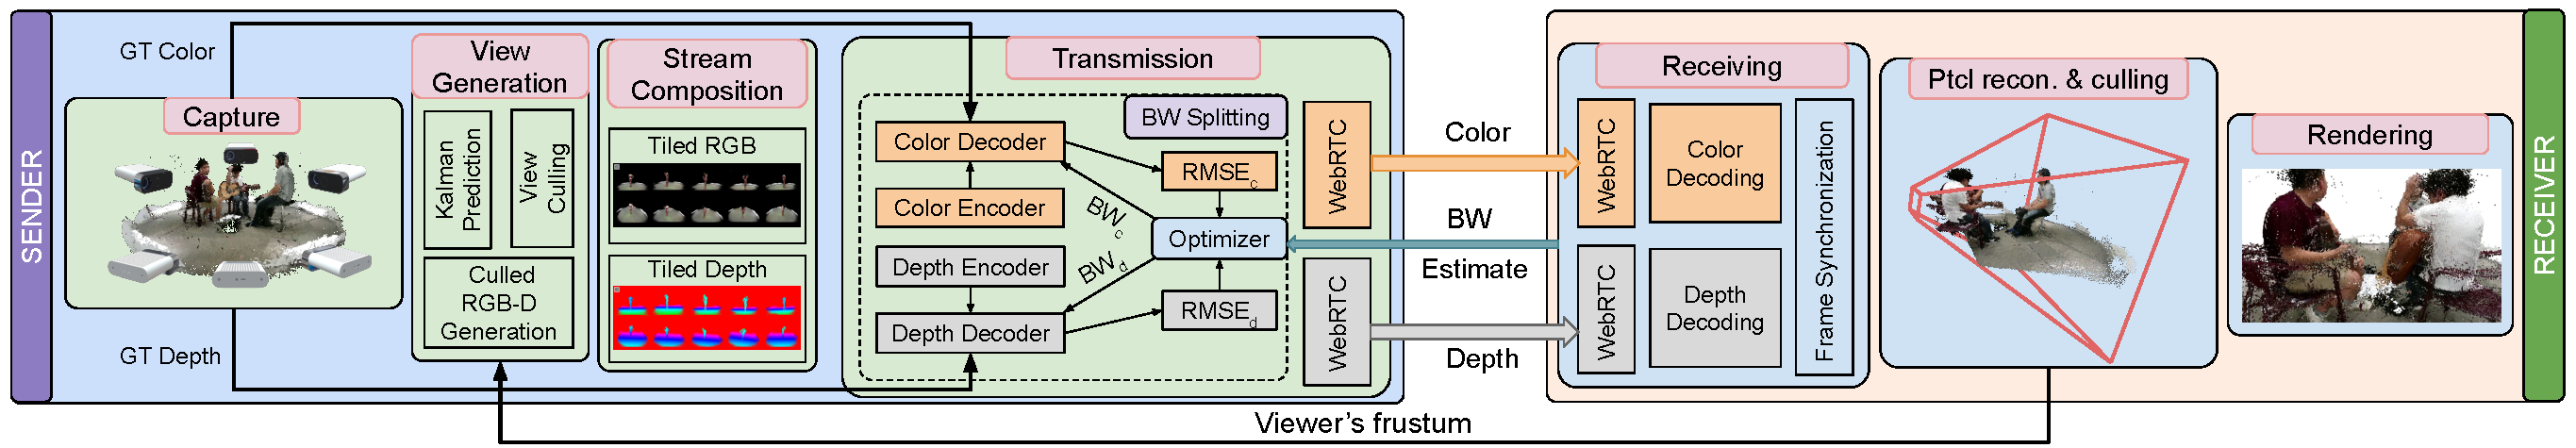
\includegraphics[width=\textwidth]{figures/Livo - Architecture New.pdf}
  \caption{\livo Architecture. The \textcolor{green}{green} blocks on the left run on the sender and \textcolor{blue}{blue} blocks on the right run on the receiver.}
  \label{fig:architecture_livo}
\end{figure*}

%\harsha{The first two paras here are a bit repetitive, given the context setup in previous section.}
\livo enables volumetric video conferencing between two sites.
%
Each site has an \textit{array} of off-the-shelf RGB-D cameras and a desktop-class computing device for processing, sending, or receiving volumetric video from the other site, as well as a viewing device (\eg a mixed reality headset).
%
Multi-way conferencing can be built using \livo, but presents opportunities for optimizations (\eg across receivers from a single sender) that we leave to future work.

\cref{fig:architecture_livo} pictorially depicts the design of \livo's sender-to-receiver pipeline; in the deployment model above, each site runs one instance of the pipeline in each direction.
%
\livo captures a sequence of RGB-D frames from each camera in an array encircling a scene (\eg a conference table, a small stage or performance area, or a small room).
%
At a given instant, a frame from each camera can be used to generate a point cloud (\cref{ss:compression}), and a sequence of successive point clouds constitutes the volumetric video.

\livo transmits the volumetric video as streams of 2D video.
%
This choice permits \livo to re-use mature widely-deployed technology:
%
(a) off-the-shelf highly efficient video compression standards such as H.264 and H.265;
%
(b) mature rate-adaptive open-source codec implementations (\eg GStreamer~\cite{gstreamer} and FFmpeg~\cite{ffmpeg});
%\antonio{Following discussion via email with Ramesh: we can use whatever term is used in Section 2, e.g., codec software with built-in rate control}
%
and (c) real-time transport for video conferencing such as WebRTC~\cite{webrtc} with its built-in Google congestion control~\cite{gcc}. 

%\sanjay{Project Starline also uses 2D video streams and we learn this later in evaluation.Would it be better to state this upfront, but then say there are many challenges that have to be addressed such as culling and bandwidth adaptation which Starline does not address and is our focus?}

The second is to \textit{cull} each point cloud to only include points that fall into the receiver's \textit{frustum}.
%
The frustum represents the receiver's 3D field of view (\cref{fig:architecture_livo}).
%
%It is shaped like a truncated pyramid.
%
%Recall that volumetric video is distinguished by interactivity along 6 degrees of freedom.
%
When the receiver is viewing the entire scene, her frustum includes the entire point cloud.
%
But, for example, if she moves closer to objects or participants in the scene, her frustum will likely include a much smaller part of the point cloud (\cref{fig:architecture_livo}). 
%\ramesh{might consider drawing a simple graph of the fraction of a point cloud from one of our traces? Can include it either here or in the view culling section?}

Together, these address the two challenges described in \cref{s:background}.
%
2D codecs employ inter-frame compression, resulting in higher bandwidth-efficiency relative to point-cloud compression.
%% \raj{2D codecs addresses 2 challenges faced by 3D codecs: bandwidth efficiency and encoding/decoding at line rate.}
%
Culling further reduces the bandwidth requirements.
%
Moreover, 2D codecs can encode to a target bandwidth, so \livo{} can directly adapt to bandwidth changes.
%
Finally, there exist mature, compute-efficient implementations of 2D codecs that can, with low latency, process video streams at full frame rate.

Even though it relies maximally on 2D video technology, \livo{}'s design poses two significant challenges: (a) how to encode RGB-D frames in 2D videos and how to adapt these to available bandwidth; (b) how to determine receiver frustum and cull views.
%% \antonio{I think i've seen both 2D and 2-D, let's use one consistently. }
%% \raj{Fixed issues: 3D instead of 3-D and 2D instead of 2-D}
%
We describe how \livo{} addresses these challenges in the rest of this section.

\subsection{2D Video Encoding}
\label{ss:compression}

\parab{Background: Point Clouds from RGB-D Camera Array.}
%
%Before describing how to encode point clouds in 2D videos, we explain how point clouds are derived from an RGB-D camera array.
%
Each camera produces RGB color and depth frames at 30 frames per second.
%
Consider a static RGB-D camera array (\cref{fig:architecture_livo}) with $N$ frame-synchronized cameras.\footnote{There exist techniques to synchronize Kinect cameras~\cite{kinect-sync}.}
%
Then, for every inter-frame interval (30th of a second), we can generate a point cloud from $N$ frames, one from each camera.
%
To do this, we need to determine the position and orientation of each RGB-D camera in a common frame of reference.
%
There exist standard one-shot calibration techniques for this~\cite{zhang-calib} that produce a transformation matrix to convert each camera's local coordinate system to a global one.
%
Generating a point cloud is then simple: for each pixel of each RGB-D frame, first determine the pixel's position in the camera's local coordinate frame (using camera parameters such as its center and focal length~\cite{metastream}), and then convert it to global coordinates (using the transformation matrix) to obtain one point in a point cloud.

%\tao{"such as its center", more precisely is "optical center"}

\parab{The Challenge.}
%
Prior work in volumetric video generates a point cloud at the sender then applies point cloud compression (\eg Draco~\cite{draco})~\cite{livescan3d, metastream}.
%
\livo{} is qualitatively different: it encodes 2D RGB-D video frames \textit{directly} at the sender, and the receiver decodes and constructs a point cloud for viewing.
%
An array of $N$ cameras produces $N$ color frames and $N$ depth frames at 30~fps.

For these frames, \livo{} must solve three distinct problems: \textit{stream composition}, \textit{depth encoding}, and \textit{bandwidth splitting}.
%
Stream composition refers to the problem of multiplexing the 2$N$ images into one or more video streams.
%
Multiplexing all images, depth and color, onto a single stream defeats inter-frame prediction because successive frames might be from different cameras or might interleave color and depth frames.
%
At the other extreme, independently encoding each camera's output into a color stream and a depth stream increases complexity in two ways.
%
First, the receiver must reassemble related color and depth frames from different streams to reconstruct the point cloud.
%
We have found this reassembly tricky, especially when different streams incur different delays.
%
Second, if \livo{} composes frames into more than one stream, it must determine how to split available bandwidth to each stream (\cref{ss:bw-adaptation}).
%
The more streams there are, the more complex the splitting algorithm.

Depth encoding converts pixel depth values into a format that video codecs recognize.
%
For example, one can encode depth in one of the three color channels (R/G/B) in a color image.
%
In general, this approach can introduce significant distortions, since video compression algorithms exploit smoothness in natural images to achieve compression, but depth information can exhibit discontinuities~\cite{depth-kautz,depth-antonio,depth-wilson}.
%
\livo{} must attempt to minimize depth distortion, especially since humans are very sensitive to point cloud depth errors~\cite{graphsim}.
%As a result, the reconstructed point cloud can have poor quality, so \livo{} must encode depth without compromising quality.

In this subsection, we describe \livo{}'s stream composition and depth encoding, then discuss bandwidth splitting in \cref{ss:bw-adaptation}.

\parab{Stream Composition.}
%
\livo leverages technology trends to compose streams in a novel way.
%
Off-the-shelf RGB-D cameras have lower depth resolution than color resolution.
%
For example, the Azure Kinect DK offers $640 \times 576$ \textit{depth} image resolution, and the Intel RealSense D457 supports up to $1280 \times 720$, but their color images can have up to 4K resolution. %\raj{The highest possible resolution for depth is $640 \times 576$ or $1280 \times 720$, but either cameras can go upto 4K for color resolution. So, we should explicitly mention the resolution bound is for depth.}
%
These cameras usually include a time of flight sensor that measures, for each pixel, the depth of that pixel.
%
The cost of these sensors have resulted in the slower growth of RGB-D camera depth resolution.

\livo exploits this observation to multiplex the 2$N$ images into \textit{two} videos: a color video and a depth video.

%% \begin{figure}[t]
%%     \begin{minipage}{\columnwidth}
%%       \centering
%%       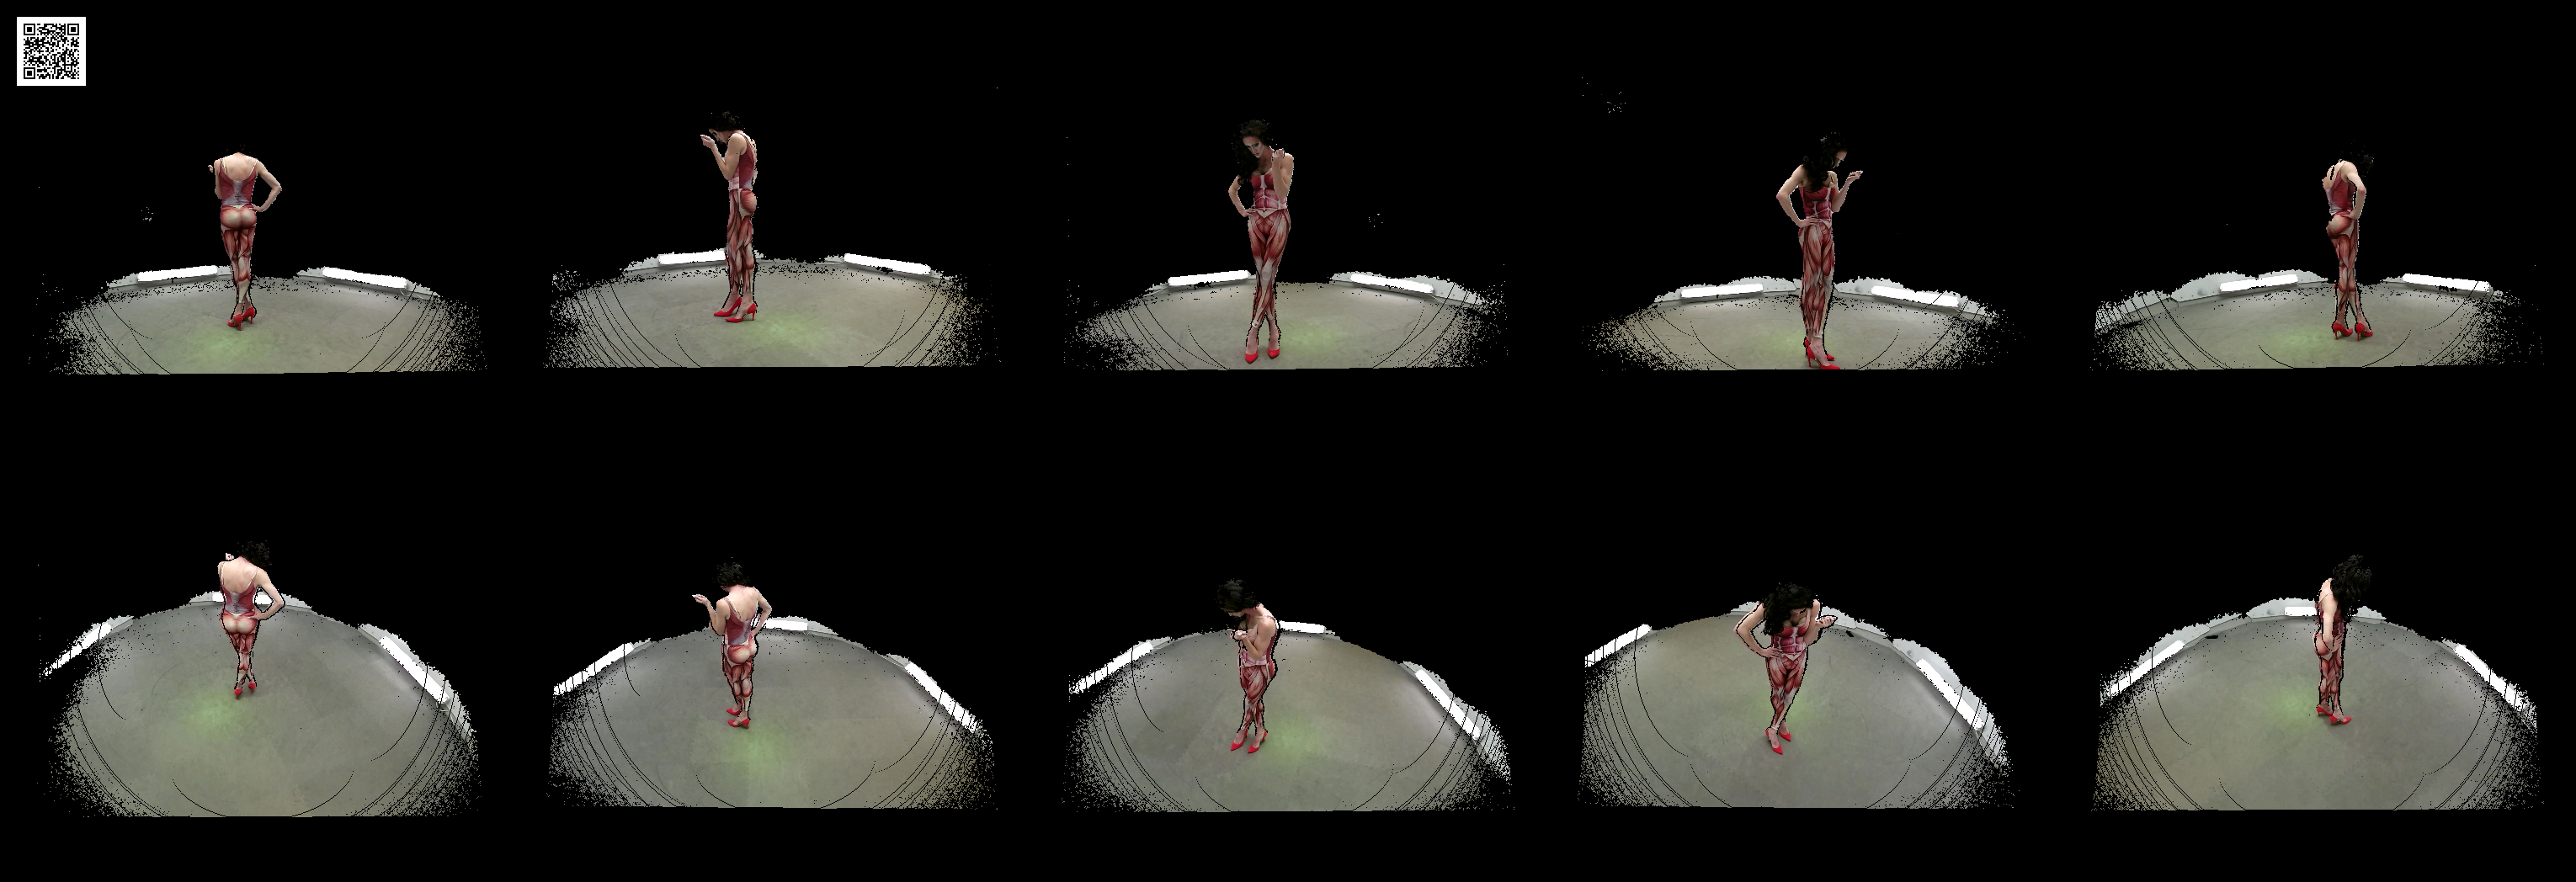
\includegraphics[width=\columnwidth]{figures/color_tiled.png}
%%     \end{minipage}
%%     \\
%%     \begin{minipage}{\columnwidth}
%%       \centering
%%       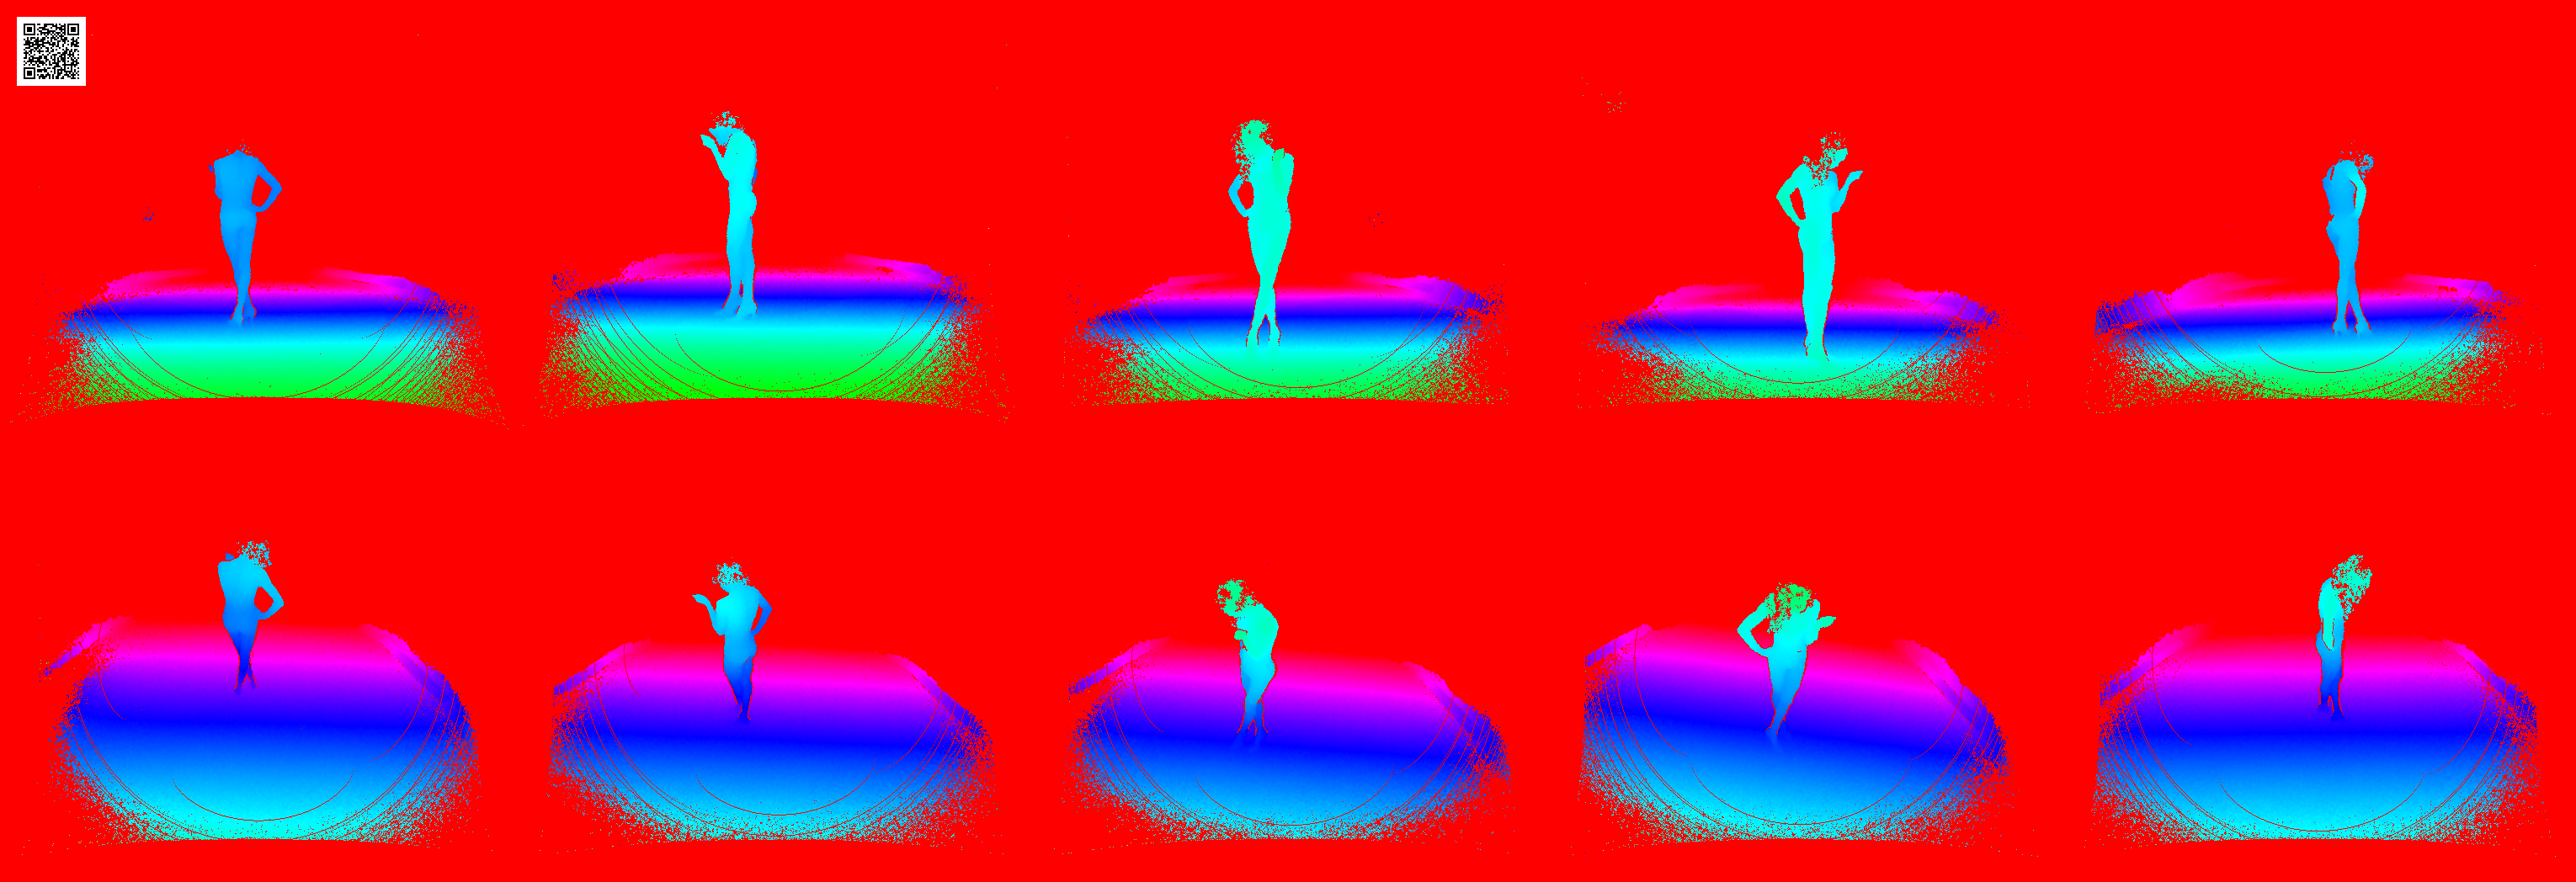
\includegraphics[width=\columnwidth]{figures/depth_tiled.png}
%%     \end{minipage}
%%     \caption{Tiled color and depth view for 10 kinect cameras. \raj{Keep only RGB as referred in the text?}}
%%     \label{fig:tiled-view}
%% \end{figure}

\begin{figure}[t]
\centering
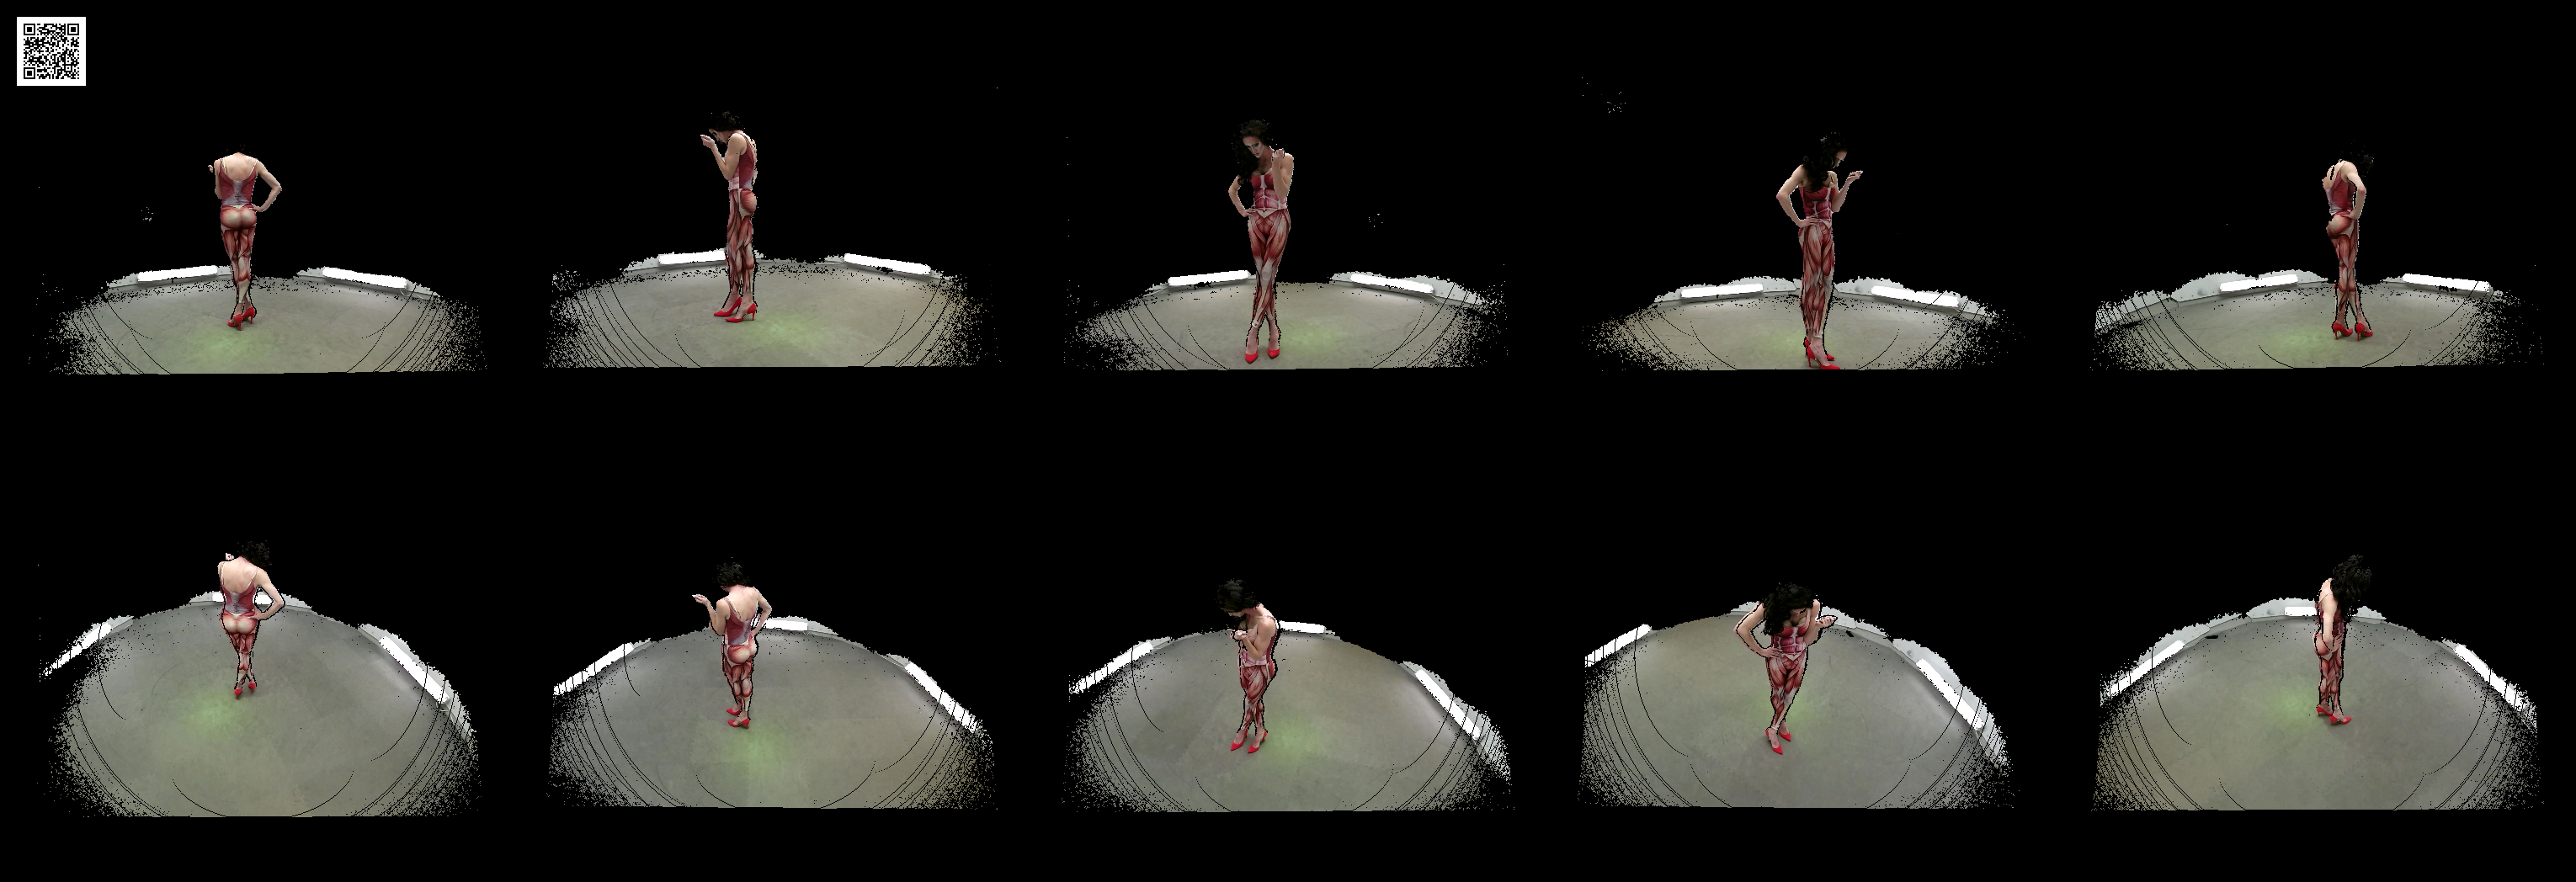
\includegraphics[width=\textwidth]{figures/color_tiled.png}
\caption{Tiled color view for 10 kinect cameras. A Similar view is generated for depth.}
\label{fig:tiled-view}
\end{figure}

Specifically, it tiles the $N$ depth images into a 4K frame (\cref{fig:tiled-view}).
%
RGB-D cameras generate color images at a much higher resolution (up to 4K), but it would be wasteful to transmit this, since the receiver would first downsample the color image to match the depth image resolution to construct the point cloud. 
%
Upsampling the depth to match color resolution is not followed in practice to avoid introducing distortion in geometry~\cite{kinect-sdk, panoptic-toolbox, livescan3d}.
%
Accordingly, \livo{} downsamples color images to the depth resolution, then tiles these downsampled color images into a 4K color frame.
%% \antonio{Downsampling potentially reduces both quality of point cloud attributes. Can we address this? If the number of points is determined by the number of pixels in the depth image, this may not have much impact. Also, are we using a direct downsampling or downsampling after filtering? If we are using as ground truth to evaluate compression the point cloud derived by downsampling the color image, this doesn't affect the result. We could include a footnote to say that this downsampling corresponds to how the point cloud attributes would be generated with a standard pipeline }
%% \raj{In \livo, we conly downsample the color to match the depth. Each pixel in depth image contributes to a point in point cloud. So this isn't an issue. And yes, this is the standard way to generate point cloud. Should we clear that in text?}
%
Using this approach, \livo can fit $9$ Intel RealSense cameras or $16$ Azure Kinect DK cameras into two 4K frames (for color and depth).
%
Given that these cameras have a modest range (5-6~m) and can only cover small spaces, we do not foresee deployments with significantly more RGB-D cameras (other work also makes similar assumptions about the number of cameras~\cite{depthkit,starline,farfetchfusion,holoportation}).
%
With more cameras, we may need to multiplex images onto more streams and add more complex receiver synchronization, which we have left to future work.

Tiling camera images consistently on a 4K frame does not impact video compression efficiency.
%
2D video codecs predict macroblocks (8x8 or 16x16 pixel blocks) within and between frames.
%
In successive frames, the location of the macroblocks is fixed (images from the same camera are located at the same spot in the tiled image).
%
Inter-frame prediction is thus relatively unaffected by tiling since the macroblocks preserve locality, improving compressibility.
%
%% Intra-frame prediction might be slightly less efficient at tile edges because a macroblock at the edge of one tile may not be able to predict a neighboring macroblock.
%% %
%% To avoid this, we add a macroblock-sized black border around each tile, which introduces a discontinuity that avoids prediction across the border.
%% %\sanjay{Why does it help? Does it turn off intra-frame prediction across the border?}
%% %
%% However, inter-frame prediction (between macroblocks at the same location in successive images) is relatively unaffected because \livo maintains tile consistency: a color (resp. depth) image from an RGB-D camera is at the same location in every 4K tile.
%% %
%% \antonio{In practice this is not a major problem. The codec automatically can switch intra prediction off if the prediction is not good. }
%

After tiling, \livo passes each color 4K image to an H.265 encoder (see below for depth).
%
These can encode 4K frames at full frame rate.
%
%\raj{Reviewer 4 had a confusion. Though depth resolution is smaller, color resolution for these cameras can go upto 4K. The confusion is depth can be tiled easily, but 4K color tiling is not scalable; tiling can only work for Panoptic but not for recent cameras. Reason for the confusion is we don't mention that point cloud generation require high resolution color frames to be downsampled to depth resolution. Since both color and depth have same resolution, our tiling can scale to any RGBD cameras available today.}

%% \ramesh{Add here the results of the experiment on encoding $2N$ streams vs 2 streams.}

% \begin{figure}[t]
%     \centering
%     \includegraphics[width=\textwidth]{example-image-duck}
%     \caption{\raj{Plot showing geometry error between depth to RGB quantization vs naive 16-bit encoding vs scaled 16-bit encoding}}
%     \label{plot:depth-encoding}
% \end{figure}

\parab{Depth Encoding.}
%
Prior work has explored two different techniques to encode depth into images.
%
One approach encodes a 16-bit depth value into a 3-channel RGB pixel~\cite{realsense-doc, depth-kautz, vrcomm}.
%
This attempts to ensure that the depth encoding respects color \textit{smoothness} so that video codecs can compress the resulting image without significant distortions.
%
This works well for shorter depth ranges (of about 1.5~m~\cite{vrcomm}) but not for larger ranges (\cite{depth-kautz}, \cref{s:evaluation}).

%% We have experimented with this, and found that it does not work well in practice (\cref{s:evaluation}). %\ramesh{Move figure to eval.}
%% \harsha{Why does depth encoding suggested by RealSense not work well for us? What's different in our setting?}
%% \raj{Converting depth to color, encoding using 2D video codec, and reconverting color to depth after decoding introduces lots of artifacts. The reason is 2D video codecs try compress by remapping similar colors to same quantization level. This is not good for depth as it is sensitive to small changes. Another work has shown this problem~\cite{depth-kautz}. A recent work~\cite{vrcomm} has used similar technique, but they only consider depth range of 1.5~m. In our full scene setting, this technique doesn't work.}

Other work~\cite{starline, farfetchfusion} encodes 10-bit depth into the Y-channel of a YUV~\cite{yuv} (a different way to represent color) encoding.
%
Codecs compress the Y-channel (representing luminance) at higher bit rates to avoid loss since humans are sensitive to luminance distortions.
%
For this line of work, this depth encoding works well because they target portrait 3D videos (of faces or upper torsos), which require a lower depth range (1-2~meters).
%
%For this line of work, this depth encoding works well because they target portrait 3D videos (of faces or upper torsos) with limited 6DoF capabilities.
%
Our RGB-D cameras output 16-bit depth values at millimeter resolution.
%
Quantizing these to 10 bits can sacrifice either depth or resolution, impacting perceived quality and impairing full 6-DoF capabilities.

%% \harsha{The main insight/takeaway doesn't quite come across in the para below.}
%% \raj{Does Antonio's comment at the end of the paragraph captures the insight? It is commented for now.}
\livo leverages a rarely-used H.265 mode, which supports a 3-channel 16-bit YUV encoding~\cite{gstreamer-nvenc}.
%
\livo stores the 16-bit depth pixel value in the Y channel and sets the U and V channels to the same fixed value.
%% \antonio{fixed values = all pixels are given the same constant value? }
%% \raj{Yes, all pixels have same constant value.}
%
This reduces depth distortion since codecs distort the Y-channel less.

However, simply storing the depth value in 16 bits on the Y channel introduces significant artifacts (\cref{fig:depth-unscaled-artifact}).
%
Current depth cameras have a maximum depth range of 5--6~meters~\cite{kinect-spec, realsense-spec}, so the depth values can range from $0-6000$ at millimeter resolution.
%
%\footnote{\livo{} communicates this range between sender and receiver during session establishment.}
%
This uses only part of the full 16-bit range.
%
%To avoid artifacts, we scale the depth value to occupy the entire 16-bit range.
Instead, we scale the depth value to occupy the entire 16-bit range, \ie scaled depth value for 0~mm remains at 0 while it is $2^{16}-1$ for 6000~mm.
%
This approach incurs lower depth distortion: codecs quantize depth values, and, for a given quantization step size, more unscaled depth values fall into one quantization bin than scaled depth values.
%
%We use a conservative depth range that works well in our setting; if camera positions change, causing depth ranges to change, \livo{} will need to change the scaling factor to reduce depth distortion.
%
%This may require a re-calibration step~\cite{metastream}, which we have left to future work.

%% \antonio{One downside of doing this per frame is that the depth distortion may change if the range of depths in the scene changes. This may not be an issue for set ups where the cameras are fixed and and there isn't much change on the scene. One downside of doing this per frame is that the depth distortion may change if the range of depths in the scene changes. This may not be an issue for set ups where the cameras are fixed and and there isn't much change on the scene.  }
%% \raj{Antonio is correct. If the camera setup changes, our solution may cause variable distortion. So, our depth encoding method needs further validation for moving camera setup.}
%% \tao{is it linearly scaled? It might be worth putting an equation if it's not linearly scaled for reproducibility purposes.}

%% \antonio{First, it's not clear if this is done per frame (I assume it is) and whether side information needs to be sent (it should be) so that decoder knows the range of values. Second, we can explain why this is better: when we expand to use the whole the quantization step size (which is fixed for a given rate) results in a smaller overall quantization. There may not be space to include this, but assuming the range is [0, Max] and we expand to [0, K*Max], where K*Max = 2^{16} - 1, then our effective quantization stepsize is $\Delta$/K rather than $\Delta$.}.

\subsection{Bandwidth Splitting}
\label{ss:bw-adaptation}

\parab{Background: WebRTC and Rate-adaptive Codecs.}
%
Unlike on-demand HTTP-based video streaming, 2D video conferencing systems use a real-time transport protocol (\eg WebRTC) with rate-based congestion control (\eg GCC~\cite{gcc}).
%
The sender feeds the available bandwidth from congestion control to a rate-adaptive video encoder, which compresses the frame to fit within the target bandwidth.

\parab{The Challenge.}
%
\livo transmits depth and color videos as two separate WebRTC streams.
%
Suppose, at a given instant, the sender's rate control algorithm estimates an available bandwidth of $B$.
%
\livo{} cannot assign $B/2$ to each stream.
%
It encodes depth (\cref{ss:compression}) to reduce depth distortion, but in order to get higher quality, it must \textit{also} assign more bandwidth to the depth stream than the color stream.
%
\figref{plot:depth_vs_color_rmse} shows the variation in quality for depth and color at different splits of a target bandwidth of 80~Mbps for one of the videos we use in \cref{s:evaluation}.
%
When the depth stream gets 90\% of the available bandwidth, the error in depth and color is lowest.
%
This is because humans are much more sensitive to depth than to color errors~\cite{graphsim}; allocating more bitrate to depth reduces depth distortion~\cite{sigcomm-ems}.
%
Moreover, distortion in depth can also distort objective measures of color quality~\cite{sigcomm-ems}.
%
% Point cloud quality metrics match distorted points to ground truth points in the 2 point clouds, then compare color between matched points.
% %
% If a pixel's depth is distorted, this can result in mismatches, adversely affecting color quality measures~\cite{sigcomm-ems}.

%% \tao{It's unclear to me what's the key reason why depth distortion produces color distortion. It sounds like you are trying to say the evaluation metric (PointSSIM) suffers from depth distortion.}

\begin{figure}[t]
  \centering 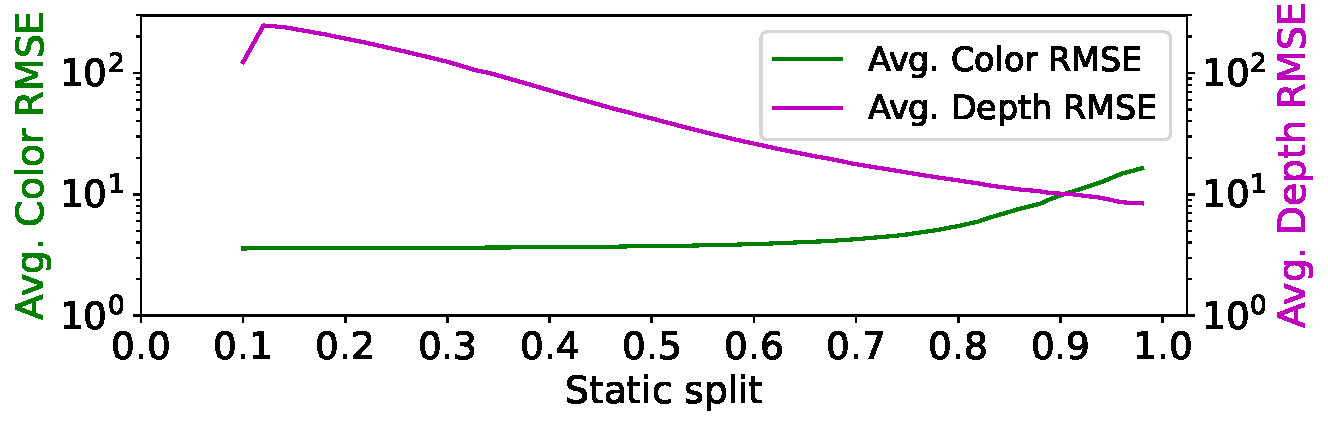
\includegraphics[width=\textwidth]{figures/color_depth_rmse_vs_split_bwe80000_logscale.pdf}
	\caption{Color and depth RMSE for different splits at target bandwidth of 80~mbps. Log-scale y-axis. Video sequence: \textit{band2}}
  \label{plot:depth_vs_color_rmse}
\end{figure}

To ensure high quality, \livo{} must determine the \textit{bandwidth split} $s$: the fraction of available bandwidth allocated to the depth stream.
%
A strawman approach might profile off-line, a collection of volumetric videos to determine an optimal \textit{static} split at a given bandwidth.
%
Intuitively, this split jointly minimizes distortion in depth and color.
%
For example, \cref{plot:depth_vs_color_rmse} suggests a split $s$ of 90\%.
%
It is an open question whether such an approach can generalize easily; the optimal split can vary from frame to frame, as \textit{scene complexity} --- the number of participants, or the degree of motion --- changes.
%
%Static splits cannot capture these.
%
It might be possible to design learned split predictors, but these might need a lot of data with varying degrees of scene complexity to generalize well, and we have left this to future work.

%% \tao{For ease of understanding, this section can benefit from adding something similar to a rate-distortion equation to show the bandwidth split of color and depth and the quality of them combined. Especially there are a couple of notations discussed throughout this entire subsection, including the bandwidth split s in the next subsection.}

\parab{Adaptively Splitting Bandwidth.} 
%
Instead of determining the split statically, \livo{} \textit{adaptively} and continuously determines splits to capture bandwidth and scene complexity changes.
%% \harsha{I assume the latter part of the previous sentence is not right?  Even if the bandwidth estimate does not change, we might need to change the split if scene complexity changes.}
%% \raj{Harsha is right. Even for same bandwidth, the split can change based on scene complexity. Split is dependent on both change in scene complexity and change in bandwidth estimate.}
%
%% \antonio{For clarity we may want to define split, i.e., the split parameter $s$ is the fraction of bandwidth allocated to depth. }
It repeatedly encodes a frame with a given split $s$, determines the resulting quality of the encoded frame, and then either increases or decreases $s$ to improve depth and color quality.
%
To do this, it must solve two problems: (a) how to estimate encoding quality and (b) how to adapt.

\parae{Estimating encoding quality.}
%
\livo{}'s approach encodes a frame at the sender, immediately decodes it, and then computes distortion with respect to the ground truth frame (available at the sender).
%% \antonio{Instead of ``compare'' which is informal, use ``compute distortion with respect to the original'', or something along those lines. }
%
Today, GPU-accelerated video encoders and decoders, like NVIDIA's \texttt{nvenc}~\cite{nvenc-sdk}, can decode multiple frames while also encoding other frames.
%
So, while the GPU is encoding a frame, it can decode a previously encoded frame to determine quality.
%
Parallel decoding minimally impacts GPU utilization.
%
%% \raj{If required, we can add GPU utilisation with and without parallel decoders. Show that the overhead is negligible.}\ramesh{Yes, this would help. Will add number once results are ready.}\tao{Desktop GPUs typically have multiple codec blocks to support multiple simultaneous streams, too.}

To estimate the quality of the decoded frames, \livo{} could use a point cloud quality metric such as PointSSIM~\cite{pointssim}, but this requires the sender to reconstruct the point clouds before and after encoding.
%
\livo{} instead uses the root-mean-square error (RMSE) in pixel values between the original (depth or color) frame and the decoded frame.
%
%% RMSE is the square root of the mean of the squared error in pixel values between the decoded image compared to the ground truth image. 
%% \antonio{previous sentence is repetitive, combine with the one before}
%
%% \tao{It is unclear to me why decoded frame quality evaluation ideally has to use PointSSIM.}
%
%% For color, it is the mean deviation of the intensity values in each channel (RGB).
%% %
%% For depth, it captures change in depth in the z-axis.
%
This choice is far more compute-efficient.
%
\livo{} further reduces the compute overhead by computing RMSE every $k$ frames ($k=3$, chosen empirically, in our evaluations, \cref{s:evaluation}), instead of every frame.

%% \tao{How is k=3 chosen? Does the intensity value mean the magnitude of data in RGB channels or the luminance in the Y channel?}

\parae{Adapting the split.}
%
\livo{} continuously adapts the split using the following steps (\cref{fig:architecture_livo}):
\begin{itemize}
\item It uses two video decoders (running parallely) which decode the compressed tiled frames to generate the distorted tiled color and depth frames.
\item For each decoded color (resp. depth) frame, it calculates the color RMSE $RMSE_c$ (resp. depth RMSE $RMSE_d$) by comparing the distorted tiled frame ($F'$) to the ground truth tiled frame ($F$).
\item \livo{} does not modify the split if $|RMSE_d - RMSE_c| \le \epsilon$, where $\epsilon$ is a parameter to the algorithm.
%% \harsha{Why the choice of $atol$ as the name?}
%% \raj{$atol$ means Absolute Tolerance. It is a common term used in optimization algorithms.}
\item It runs multi-dimensional line search~\cite{linesearch-hauser,linesearch-bookchapter} to find this optimal split. This additively increases or decreases $s$. If $RMSE_d - RMSE_c > \epsilon$, then $s$ increases by $\delta$ (the step size). Else, $s$ decreases by $\delta$.
\end{itemize} % Ensure proper closure of the itemize environment

%% \antonio{Previously we used $s$ for split. I'm not a big fan of using words for variables. How about $s$, $s_0$ for the initial value of the split and $s_t$ for the split at time $t$?}
%% \raj{Should we do $csplit$ as $s_t$, $isplit$ as $s_0$?}

At the beginning of a session, $s$ is set to an initial split $s_i$.
%
This can be estimated empirically from video data (\eg \cref{plot:depth_vs_color_rmse}) or can be set to a fixed initial value.
%
%% In each frame, \livo{} assigns the bitrate based on $csplit$;~\algoref{algo:bitrate-split}.
%% %
%% A separate thread updates the $csplit$ based on the algorithm in~\algoref{algo:bitrate-split-adapt}.
%% %
%% Since RMSE can be easily calculated, we observe that the split can be updated as fast as half the frame rate.
%% \harsha{Not sure what previous sentence means.}
%% \raj{The previous sentence means that the split can be updated every 2 frames.}

Multi-dimensional line search is sensitive to $\delta$.
%
A smaller value can lead to delayed convergence when the scene complexity changes.
%
A larger step size can result in oscillations around the optimal split.
%
We have empirically chosen a step size of $0.005$ to balance these two concerns.
%

We also choose  $0.5 \leq s \leq 0.9$.
%
The lower limit ensures depth always gets more bandwidth than color.
%
%The choice of 0.9 prevents degenerate behavior under low bandwidth conditions.
%
When available bandwidth is too low, $RMSE_d - RMSE_c$ may always exceed $\epsilon$, which will drive $s$ to 1, and this can degrade color significantly. %
%
To prevent this, we clamp $s$ at 0.9.

%% \tao{This is the interesting part of the paper. However, I do not see a block diagram showcasing your system design regarding adaptive splitting of bandwidth. Figure 2 is relatively high-level and does not include adaptive splitting.}

%% \begin{algorithm}[h]
%% % \footnotesize
%%   \caption{Bitrate Splitting}
%%   \label{algo:bitrate-split}
%% \SetAlgoLined
%% \DontPrintSemicolon    % Remove semicolons at end of lines (optional)

%% \SetKwInOut{Input}{Input}
%% \SetKwInOut{Output}{Output}

%% \Input{Target Bandwidth $B$, Initial split $isplit$}
%% \Output{Color Bitrate $B_c$, Depth Bitrate $B_d$}
%% \BlankLine

%% \textbf{Initialize:} $csplit \gets isplit$\;
%% % Allocate target bitrate $B$ to depth and color according to $csplit$\;
%% $B_d \gets csplit \times B$ \tcp*{Depth bitrate}
%% $B_c \gets B - B_d$   \tcp*{Color bitrate}
%% \Return $B_c, B_d$\;

%% \end{algorithm}

%% \begin{algorithm}[h]
%% % \footnotesize
%%   \caption{Bitrate Split Adaptation}
%%   \label{algo:bitrate-split-adapt}
%% \SetAlgoLined
%% \DontPrintSemicolon

%% \SetKwFunction{TimeSynchronization}{TimeSynchronization}
%% \SetKwFunction{ColorDecode}{ColorDecode}
%% \SetKwFunction{DepthDecode}{DepthDecode}
%% \SetKwFunction{ColorRMSE}{ColorRMSE}
%% \SetKwFunction{DepthRMSE}{DepthRMSE}
%% \SetKwFunction{Clamp}{Clamp}

%% \SetKwInOut{Input}{Input}
%% \SetKwInOut{Output}{Output}

%% \Input{GT Color $F_c$, GT Depth $F_d$}
%% \Output{Current Split $csplit$}
%% \BlankLine

%% % Pair of decoders (color and depth) decode tiled frames on the sender.\;
%% % Occasionally, estimate 2D color RMSE ($cRMSE$) and depth RMSE ($dRMSE$)
%% % between the decoded tiled frames and the ground truth.\;

%% $F_c' \gets $ \ColorDecode { }\;
%% $F_d' \gets $ \DepthDecode { }\;

%% $RMSE_c \gets $ \ColorRMSE {$F_c$, $F_c'$}\;
%% $RMSE_d \gets $ \DepthRMSE {$F_d$, $F_d'$}\;

%% $\delta \gets RMSE_d - RMSE_c$\;
%% \If{$|\delta| \le atol$}{
%%    \Return $csplit$\;
%% }
%% $csplit \gets csplit + (\text{STEP\_SIZE}) \times \delta$\;
%% $csplit \gets $ \Clamp {$csplit$, $0.5$, $0.9$}\;
%% \Return $csplit$\;

%% \end{algorithm}

\subsection{View Prediction and Culling}
\label{ss:view-prediction-and-culling}

In addition to encoding RGB-D frames in 2D video, \livo{} \textit{culls} points that are not in the receiver's view.
%
To do this, it must (a) determine the receiver's \textit{frustum} and (b) efficiently remove points outside the frustum.

\parab{Challenge: Frustum Prediction.}
%
The frustum is determined by the pose (position and orientation) of the receiver's headset, as well as the parameters of the viewing device (such as the focal length and aspect ratio).
%
Today's headsets can provide continuously evolving values for these, and the receiver can transmit these to the sender.
%
Even so, given the feedback delay between the receiver and the sender, the latter must \textit{predict} the frustum of the receiver at the time when the receiver views the frame.

On-demand 360-degree video systems~\cite{flare, dragonfly} train viewport predictors from user data.
%
In that setting, if many users watch the same video, learned predictors can be accurate.
%
In a conferencing setting, it is less clear if learned predictors can be accurate, since each conference call is unique and not enough user traces might be available for the same content.
%
We show (\cref{s:evaluation}) that predictors trained from a few traces perform poorly relative to \livo{}'s approach.

%Prediction is qualitatively harder for volumetric video, since
%receivers have 6 degrees of freedom (position and rotation) instead of 3 degrees of freedom (rotation only for the viewport in 360-video).
%
%\harsha{I'm a bit confused: after saying above that frustum prediction is a challenge, we appear to be saying below that it is not really that hard because of low end-to-end latency.}
%\rn{I guess the point is that the low latency means we can predict over very short timescales?}
%
%However, with low end-to-end latency and, therefore, smaller prediction horizons, it may be possible to \textit{accurately} predict receiver frustums cheaply, an observation \livo{} exploits.
%
%\rn{low latency means shorter prediction horizon, right? I initially read it more so as faster feedback. More importantly, isn't the low latency also true for viewport prediction?}

%
\begin{figure}[t]
  \centering
  \begin{subfigure}[t]{0.49\textwidth}
    \centering
    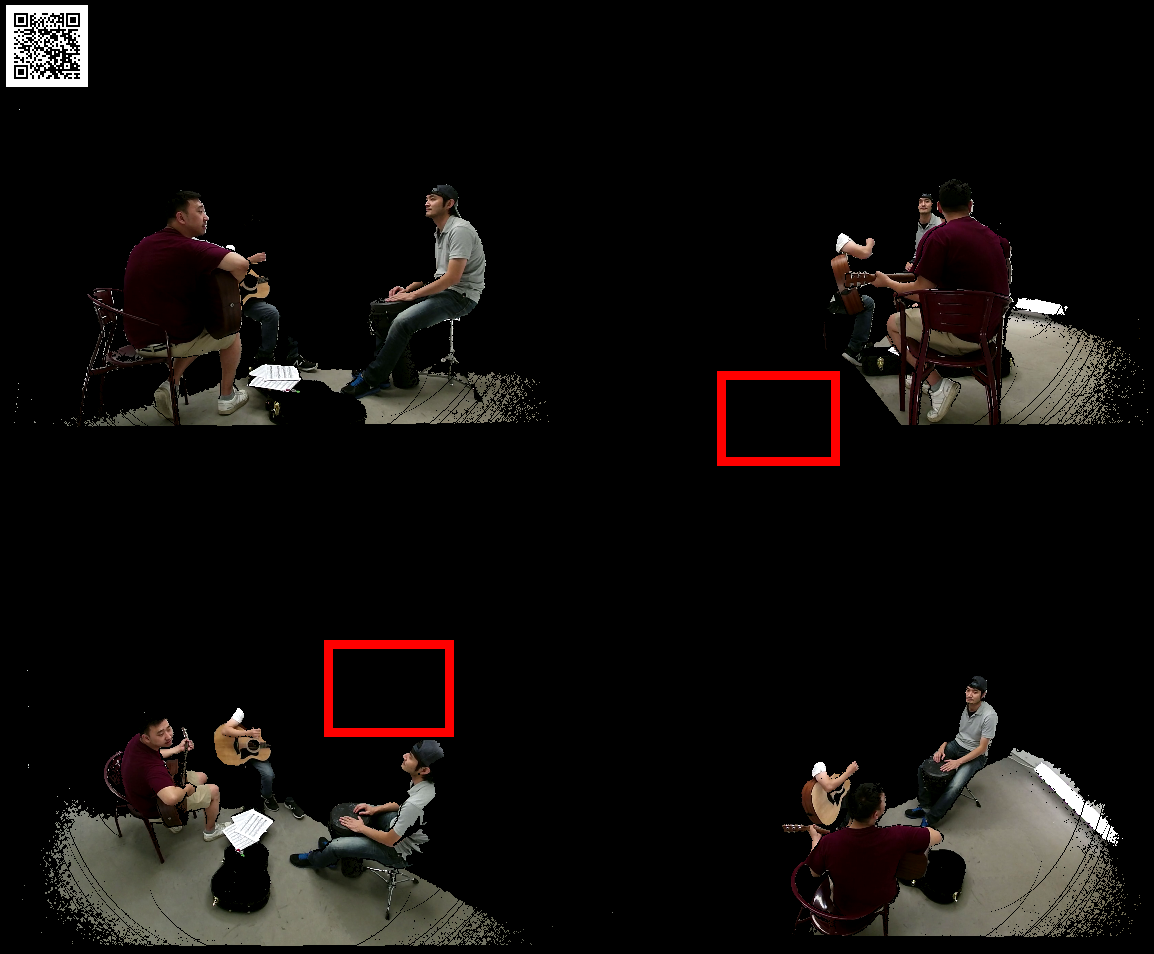
\includegraphics[width=\textwidth]{figures/10_color_bgra.png}
    \label{fig:tile1}
  \end{subfigure}
  \hfill
  \begin{subfigure}[t]{0.49\textwidth}
    \centering
    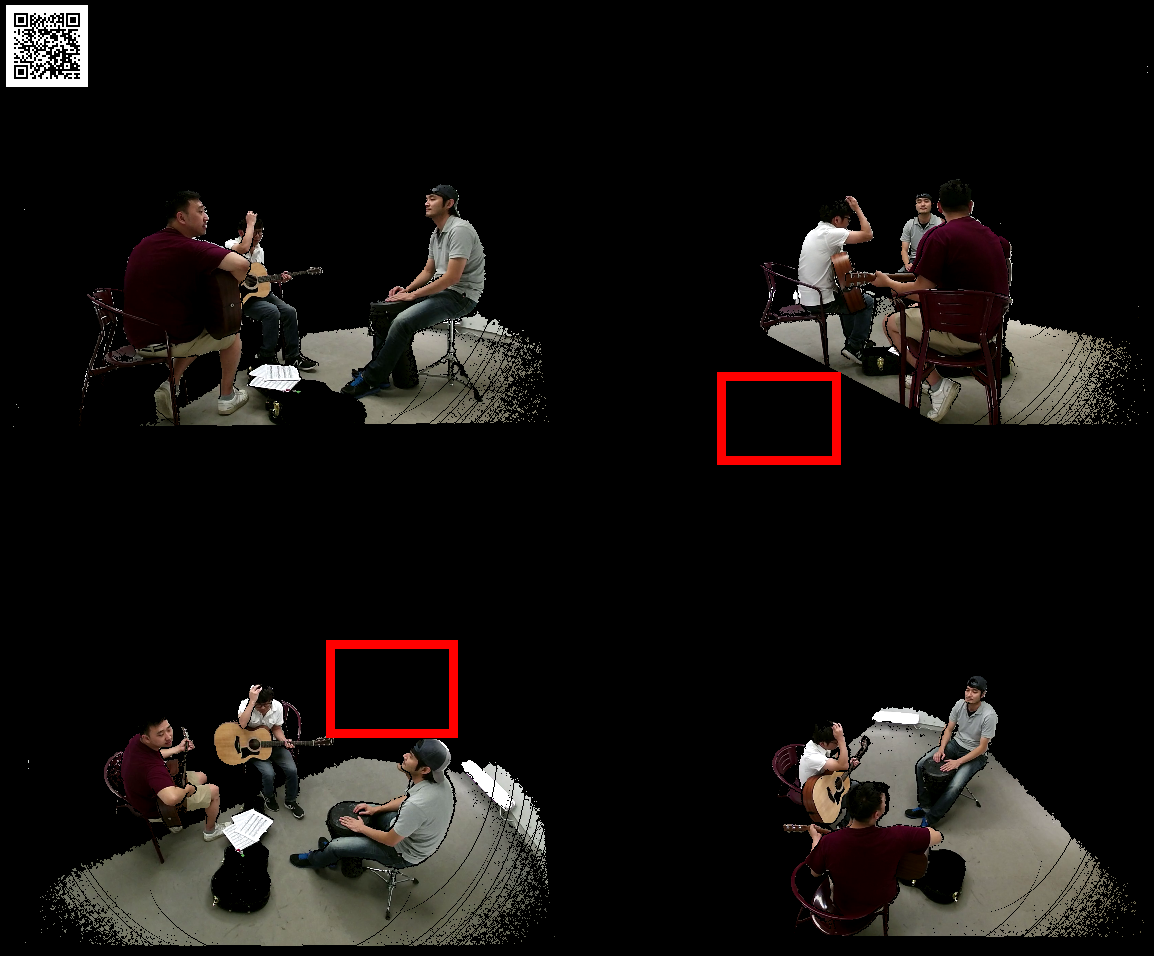
\includegraphics[width=\textwidth]{figures/20_color_bgra.png}
    \label{fig:tile2}
  \end{subfigure}
  \caption{The \textcolor{red}{red} boxes are culled regions with black pixels in two successive tiles that video encoders can compress efficiently.}
  \label{fig:cull-compress}
\end{figure}

\parab{Challenge: Efficient Culling.}
%
Given a frustum and a point cloud, the \textit{culled point cloud} consists of points inside the frustum.
%
However, RGB-D cameras do not provide point clouds; each camera produces an image, with color and depth of associated pixels.
%
\livo{} must efficiently determine which color and depth pixels correspond to points within the frustum.

%% \raj{2 Reviewers: Why we don't use learning based predicition methods (sofisticated) as opposed to Kalman Filter (simple). 
	
%% 	Learning based predicitons are suitable for on-demand streaming~\cite{vivo, vues} since they can collect user traces to train a model for prediciton. Video conferencing is a use-only-once scenario, where the content is viewed live. Learning based models trained on past user traces from conferencing, may not generalize well in future due to change in the saliency of the content. Also, this results in a cold-start issue when past user traces aren't available for a new RGB-D camera setup. Kalman Filter is a better choice since it can learn online and is only dependent on the user trace of the ongoing session.}


\parab{Frustum Prediction.}
%  
When culling a frame at time $t$, \livo's sender must predict the receiver's frustum at $t+\Delta t$, where $\Delta t$ is the one-way delay from sender to receiver (including both network and processing delays at the two ends).
%
\livo obtains $\Delta t$ by halving a smoothed application-level RTT estimate.

\livo{} predicts frustums using a Kalman Filter~\cite{kalman-original} on the 6 dimensions of receiver pose (position and orientation)~\cite{kalman-filter-mm}.
%
Still, prediction errors can arise as a result of sudden user movement or errors in one-way delay estimates.
%
To counter these, \livo expands the predicted frustum by a guard-band of $\epsilon$.
%
We have found an $\epsilon$ of 20~cm to be the sweet spot in the trade-off between compression efficiency and reconstruction accuracy (\cref{s:evaluation}).
%
Future work can explore other techniques to ensure better tracking accuracy.

%%   Accurate view prediction

%%   \squishlist
%% \item Introduce Kalman Filter
%% \item \textbf{(novel)} Frustum estimation from Kalman filter.
%%   \squishend

%%   *********************************************
%%   \raj{Asked @christina to fill this subsection.}

%%   To reduce the data volume, \livo culls points outside the
%%   receiver’s frustum and sends this culled view only to the receiver. As
%%   a sender side, \livo needs to accurately predict the receiver’s
%%   frustum given the receiver’s previous 6DoF poses. For this frustum
%%   prediction, \livo adapts kalman filter which is an algorithm to
%%   estimate unknown variables considering series of previous measurements
%%   and noise statistically. While kalman filter is actively adopted in
%%   robot pose estimations, \livo aims to obtain a estimated frustum.

%%   \livo initializes and updates a kalman filter model with the
%%   sender’s 6DoF poses (\eg x, y, z, and Quaternion rotations) at a frame
%%   $t$, and estimates the next 6DoF poses of the sender side at a frame
%%   $t+w$ where $w$ is the window size of predictions. Then, \livo
%%   obtains a viewing frustum given the predicted 6DoF pose and camera
%%   models (\eg near and far planes) of the receiver side
%%   (\figref{fig:dummy_calc_frstm}). \christina{Do we need to put more
%%     mathematical details on how we obtain the frustum?}

%%   We observed that our kalman filter is able to predict the receiver’s
%%   frustum most of the time, but a small miss prediction (especially in
%%   rotations) can incur the significant viewing quality loss. To tackle
%%   the issue, \livo expands the predicted frustum by moving 6 planes
%%   of aht frustums outward in $d$~cm (“buffering”). We carefully analyzed
%%   the size of expansion, receiver’s viewing quality, and culled data
%%   volume, and choose the optimal $t$ given our kalman filter’s
%%   prediction window size $w$. Finally, \livo culls out the points
%%   which are outside of this predicted and expanded frustum. With this
%%   frustum culling, \livo was able to reduce the size of data volume
%%   by upto 60\%.

%% \begin{figure}[t]
%%     \centering
%%     %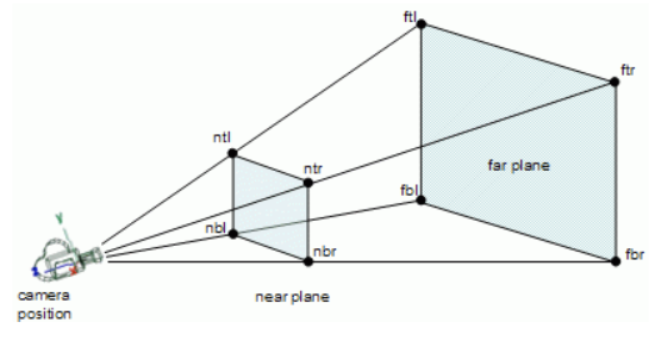
\includegraphics[width=0.8\columnwidth]{figures/dummy_calc_frustum.png}
%%     \includegraphics[width=0.8\columnwidth]{example-image-duck}
%%     \caption{Dummy figure to show how we calculate the frustum given
%%     6DoF pose and camera models. \raj{No need for this figure?}} \label{fig:dummy_calc_frstm}
%% \end{figure}

\parab{View Culling.}
This step, performed \textit{before} stream composition and depth encoding (\cref{ss:compression}), is invoked every inter-frame interval, and takes as input the viewer's frustum and the $N$ RGB-D frames.
%
For each pixel in each image, it must determine if that pixel falls within the frustum or not, and replace culled pixels by a zero value (both for color and depth).
%
%If not, it replaces the culled pixel by a zero value (for both color and depth).
%(we explain how this is produced in \cref{ss:view-prediction}) 
%and removes points not within the viewer's frustum takes as input the frustum (we explain how this is produced in \cref{ss:view-prediction}) and the $N$ RGB-D frames.
%
% Because \livo uses 2D video compression, for each RGB-D frame, view culling outputs a \textit{color image} and a \textit{depth image}.
% %
% In each, \livo represents a culled pixel by a zero value (for both color and depth).
% %
% (Somewhat better performance might be obtained if we use the average color and the average depth instead of zero, but this incurs additional compute, so we have left this to future work).
% %
% Thus, this step produces $2N$ images.
%
%This step is performed \textit{before} stream composition and depth encoding (\cref{ss:compression}). 

It can do this by (a) generating the point cloud, (b) determining whether a point is within the frustum or not and (c) back-project points within the frustum to the relevant camera's pixel.
%
This can be slow.

% Given this, a simple approach to view culling involves the following steps:
% \begin{itemize}
% \item Generate the point cloud as described in \cref{ss:compression}.
% \item For each point, determine if it is within the frustum or not.
% \item Transform (\ie back-project) every point not within the frustum back into the relevant camera's local coordinate system, and zero out the corresponding pixels.
% \end{itemize}
% %Because this operation is invoked on every frame, it needs to be fast.
% Since this culling technique requires constructing a point cloud for every frame, it can be slow.
% %
% So, \livo uses an optimized culling technique.

%% At its core, culling must determine if a point $P$ lies outside the frustum.
%% %
%% A frustum is a 3D truncated pyramid defined by size planes~---~near, far, top, bottom, left and right~---~with their plane normals pointing inwards.
%% %
%% $P$ is inside or on the frustum if the distance of the point from the six planes is non-negative, \ie the point lies in the direction of the six normals of the planes.
%% %
%% Otherwise it is outside the frustum.

\livo speeds up culling by avoiding two coordinate transformations required for each point: from local to global coordinates before culling and vice-versa after.
%
Instead, it \textit{converts the frustum into the local coordinate system} of each RGB-D camera.
%% \anotnio{Neat idea.}
%
Then, for each pixel, it obtains that pixel's local coordinates and determines if it lies within the frustum; if not, it zeroes out the color and depth of the pixel.
%
%Thus, \livo{} avoids constructing a whole point cloud and instead only uses pixel value in RGB-D for culling.


%%   \livo can stream full RGB-D views, captured from the cameras, over the network. This approach can leverage the high compression offered by the 2D video encoder. We argue that this results in unnecessary transmission of data, since the viewer can only view part of the captured scene that lies inside the FoV of the rendering device. For example, the viewer inside a scene in 6-DoF the entire scene doesn't fall inside the frustum, thus rendering the remaining scene outside the viewport is redundant. \livo can choose not to transmit this redundant data. This can either benefit in reducing the required data rate or stream RGB-D views at a higher quality by trading-off unnecessary data for higher bitrate. This leads to the question -- how can \livo cull unnecessary data from 2D RGB-D views?

%%   \livo projects each RGB-D view for a frame\_id to generate a point cloud using intrinsics of it's captured camera. Given a depth pixel value $d$ at a pixel position $<u, v>$, the pixel is projected to it's 3D location $p = <x, y, z>$ using the following relation:
%%   \begin{equation}
%%     x = (c_x - u) * z / f_x, ~~
%%     y = (c_y - v) * z / f_y, ~~
%%     z = d \label{eq:1}
%%   \end{equation}
%%   Here, $<c_x, c_y>$ is the center of the camera and $<f_x, f_y>$ are the focal length in $x$ and $y$-axes. The point with position $<x, y, z>$ is in the camera's local coordinate system. This point is projected in the world coordinate system to a position $P = <X, Y, Z>$ by transforming using the rotation matrix $R$ and translation vector $t$ obtained from the extrinsic camera matrix for the same camera using the following relation:
%%   \begin{equation}
%%     P = Rp + t  \label{eq:2}
%%   \end{equation}

%%   The RGB pixel value is an attribute associated with each point in world coordinates to form a color point cloud.

%%   Given the predicted frustum for the same frame\_id obtained from our Kalman Predictor (\secref{ss:view-predicition}), the point $P$ is culled if it lies outside the frustum. A frustum is a 3D truncated pyramid defined by size planes - near, far, top, bottom, left and right, with their plane normals pointing inwards. The point $P$ is considered inside or on the frustum, if the distance of the point from the six planes of the frustum is non-negative, \ie the point lies in the direction of the six normals of the planes, otherwise the point is considered outside the frustum. For each point obtained from $N$ RGB-D views in the world coordinates, the point is culled if it lies outside of the predicted frustum.

%%   \begin{figure}[t]
%%     \centering
%%     \includegraphics[width=\textwidth]{example-image-duck}
%%     \caption{\raj{Sender-side frustum culling and view generation.}}
%%     \label{fig:generated-view}
%%   \end{figure}

%%   Intrinsic and extrinsic camera matrix for each camera projects a pixel in RGB-D space to 3D world coordinates. Since this is a linear transformation, the 3D point that survives culling can be projected back to it's original pixel location by inversion; we call this step as \textit{back-projection}. A 3D point in world coordinates is back-projected to it's original depth pixel location with original depth value to form a new depth view, while the color information is back-projected to the same pixel location (color and depth have same resolution and pixel correspondences) with original color pixel value to form the new color view. The pixels that correspond to the culled points are replaced with depth as $0$ and color as all black ($RGB = (0, 0, 0)$) pixels. An example of 2D view generation with culling is shown in~\figref{fig:generated-view}.

%% \subsection{Other Details}
%% \label{ss:optimizations}

% \parab{Other Design Details (\cref{ss:optimizations}).}
% %
% Like~\cite{salsify}, we embed QR codes in frames to extract sequence numbers.
% %
% At the receiver, \livo{} speeds up rendering by voxelizing the point cloud.
% %
% It pipelines computation stages to achieve 30~fps, and adjusts socket buffer settings to minimize loss.

\subsection{Other Details}
\label{ss:optimizations}

Our \livo{} implementation combines techniques from various sources to achieve high-quality, low-latency volumetric video streaming. We describe these briefly.

\parab{Stream Synchronization.}
%
WebRTC does not permit embedding frame numbers in video streams.
%
Following prior work~\cite{salsify}, the \livo{} sender embeds a (pre-generated) QR code in each 4K depth and color tiled frame that encodes the frame sequence number (\cref{fig:tiled-view}).
%
The receiver decodes the QR code to obtain frame sequence numbers.
%
If both depth and color frames have not been decoded by the time necessary to render the point cloud, \livo{} simply skips the frame.

\parab{Receiver-side rendering.}
%
The receiver must reconstruct point clouds from received 4K frames.
%
To do this, it needs the parameters and positions of the RGB-D cameras; these are exchanged once during connection setup or whenever they change.
%
The receiver uses these to transform the position of each pixel from each 4K frame into the global coordinate frame.
%
Together with the corresponding color attributes, these constitute the reconstructed point cloud at the receiver.
%
This point cloud may be more dense than necessary and may have more points because \livo{} transmits a guard-band around the frustum (\cref{ss:view-prediction-and-culling}).
%
To speed up rendering, \livo{} first voxelizes the point cloud, then culls the point cloud further to the actual (current) frustum, following prior work~\cite{vivo,groot}.

\parab{Pipelining and parallelism.}
%
To ensure frame-rate processing, \livo{} consists of several stages that run in parallel, and each stage incurs a delay per frame of less than one inter-frame interval.
%
The sender has 4 stages: capture, view generation, tiling, and transmission.
The receiver also has 3 stages: receiving and synchronization, point cloud reconstruction, and rendering.
%
%% \raj{We say culling in receiver. This culling is receiver side culling to remove redundant points sent due to guard band before rendering. The audience might be confused if we suddenly say culling in receiver. May be not say about culling in the receiver? Only call the stage `point cloud reconstruction'.}
%
Thus, the total end-to-end \textit{processing} latency is within 180~ms.
%
Each stage has a dedicated thread, which is connected to the next stage by a small inter-stage buffer (implemented using a thread-safe queue).
%
We also employ parallelism within some stages when possible: \textit{e.g.}, view generation, and point cloud generation.

\parab{Minimizing the impact of packet loss.}
%
We enable several WebRTC features, including negative acknowledgments, Picture Loss Indication (PLI), and Full Intraframe Request (FIR).
%
Because 4K videos are large, the default Linux UDP socket buffer (213~KB) proved insufficient, so we increased it.

%
%\cref{ss:optimizations} describes these in detail.

%% \parab{Stream Synchronization.}
%% %
%% WebRTC does not permit embedding frame numbers in video streams.
%% %
%% Following prior work~\cite{salsify}, the \livo{} sender embeds a (pre-generated) QR code in each 4K depth and color tiled frame that encodes the frame sequence number (\cref{fig:tiled-view}).
%% %
%% The receiver decodes the QR code to obtain frame sequence numbers.
%% %
%% If both depth and color frames have not been decoded by the time necessary to render the point cloud, \livo{} simply skips the frame.

%% \parab{Receiver-side rendering.}
%% %
%% The receiver must reconstruct point clouds from received 4K frames.
%% %
%% To do this, it needs the parameters and positions of the RGB-D cameras; these are exchanged once during connection setup or whenever they change.
%% %
%% The receiver uses these to transform the position of each pixel from each 4K frame into the global coordinate frame.
%% %
%% Together with the corresponding color attributes, these constitute the reconstructed point cloud at the receiver.
%% %
%% This point cloud may be more dense than necessary and may have more points because \livo{} transmits a guard-band around the frustum (\cref{ss:view-prediction-and-culling}).
%% %
%% To speed up rendering, \livo{} first voxelizes the point cloud, then culls the point cloud further to the actual (current) frustum, following prior work~\cite{vivo,groot}.

%% \parab{Pipelining and parallelism.}
%% %
%% To ensure frame-rate processing, \livo{} consists of several stages that run in parallel, and each stage incurs a delay per frame of less than one inter-frame interval.
%% %
%% The sender has 4 stages: capture, view generation, tiling, and transmission.
%% The receiver also has 3 stages: receiving and synchronization, point cloud reconstruction, and rendering.
%% %
%% %% \raj{We say culling in receiver. This culling is receiver side culling to remove redundant points sent due to guard band before rendering. The audience might be confused if we suddenly say culling in receiver. May be not say about culling in the receiver? Only call the stage `point cloud reconstruction'.}
%% %
%% Thus, the total end-to-end \textit{processing} latency is within 180~ms.
%% %
%% Each stage has a dedicated thread, which is connected to the next stage by a small inter-stage buffer (implemented using a thread-safe queue).
%% %
%% We also employ parallelism within some stages when possible: \textit{e.g.}, view generation, and point cloud generation.

%% \parab{Minimizing the impact of packet loss.}
%% %
%% We enable several WebRTC features, including negative acknowledgments, Picture Loss Indication (PLI), and Full Intraframe Request (FIR).
%% %
%% Because 4K videos are large, the default Linux UDP socket buffer (213~KB) proved insufficient, so we increased it.

%%   Performance and quality optimizations
%%   \squishlist
%% \item View synchronization
%% \item Also need to do culling to reduce rendering time. Frustum culling -> inspired from GROOT and Vivo.
%% \item Static voxelization culling
%% \item Threading/parallelism
%% \item Mask transmission (deprecated).
%% \item WebRTC retransmissions and UDP buffer size.
%% \item QR code based frame id transmission.
%%   \squishend
%%   ********************************************

%%   \parab{View synchronization.} 
%%   The receiver decodes the received color and depth bitstreams using 2 different H.265 decoders. After depth decoding, there is an extra step to extract the single channel depth image from the Y channel and descale each pixel to $0 - 6000$~mm range. The receiver synchronizes the tiled color and depth views based on the frame\_id. This is achieved by the WebRTC thread storing the tiled frames in two small zero-copy buffer, one each for color and depth. A polling thread tries to synchronously poll a color and depth tile for a frame\_id at the desired pipeline frame rate. If either of the color or depth view for the required frame\_id isn't located in the receive buffers, the frame\_id is skipped and polling thread waits for $1/\mbox{fps}$~ms. If the synchronized views are located, the pointer to views are handed over to the ptcl generation thread, then the polling thread increments the frame\_id and waits for $1/\mbox{fps}$~ms.

%%   \parab{Ptcl reconstruction.}
%%   The receiver extracts the $N$ RGB-D views from the tiled color and depth view. Every depth pixel is projected to the local camera coordinated given by~\eqref{eq:1}, then transformed to the world coordinates given by~\eqref{eq:2}. Since the color and depth are transformed into same resolution (after capture), the color attribute is added to this point by copying the color pixel from same pixel location as the depth pixel. We represent the reconstructed point cloud as a simple array (pre-allocated memory at the start of the session) of 3D points for fast index-based operations.

%%   Frustum culling has been an essential technique to reduce rendering time in any real-time graphics rendering pipeline~\cite{cite:real-time-rendering-book}. It removes points that won't be visible to the viewer, since they lie outside the FoV based on the viewer's 6DoF position. The predicted frustum on the server captures more number of points than the actual receiver-side frustum, so we again perform frustum culling to reduce number of the points further. Unlike the server, the receiver-side culling reduces rendering latency. Volumetric video streaming systems such as ViVo~\cite{cite:vivo} and GROOT~\cite{cite:groot} have used this technique.

%%   \parab{Voxelixation-based frustum culling}
%%   Frustum culling requires checking if the distance of each point from 6 frustum planes is positive, \ie the point lies in the direction of the plane normals which are pointing inwards. The latency for culling scales linearly with the number of points. At start of the session, we voxelize the space of $6m \times 6m \times 6m$ in and around the captured scene into voxel of size $50cm \times 50cm \times 50cm$ which are axis-aligned~\cite{cite:aabb}. Naive frustum culling tests each voxel to lie within the frustum using axis-aligned object culling~\cite{cite:aabb-culling}. Instead we use a greedy technique that tests only voxels which have points in them to lie inside or outside the frustum. This method reduces the frustum culling time from testing each point to testing each voxel. Another optimization is to perform frustum culling while building a octree, where an octree node is subdivided only when the node lies on one of the frustum planes~\cite{cite:groot, cite:real-time-rendering-book}. This technique requires building the octree in real-time which has worst-case complexity worse than single level voxelization-based culling (single-level kd-tree). 

%%   \parab{Threading and parallelism.}
%%   \livo is implemented in a pipelined fashion by carefully selecting stages that can run in parallel at <$1/\mbox{fps}$~ms. We divide the sender side into 3 stages - capture, view generation, and transmission, while the receiver-side is divided into 3 stages - receiving, ptcl reconstruction and culling, and rendering. Each stage has a dedicated thread, which is connected to the next stage by a small inter-stage buffer (implemented using a thread-safe queue). For example, the capture thread pulls a RGB-D frame from the camera and adds a pointer to the frame in the inter-stage buffer. The view generation thread polls the pointer to RGB-D frame from the buffer, generates the culled view and add the pointer to the output buffer. Thus, every stage polls pointer to the data from the inter-stage buffer, performs processing and adds the pointer to processed data to the buffer, then polls the next data. We also employ parallel processing within a stage by firing OpenMP threads on loops, \eg view generation, and ptcl generation.

%%   \parab{QR-code based frame\_id transmission.}
%%   WebRTC do not support transmission of metadata such as frame\_id through video channel (WebRTC PeerConnection). The data channel can be used to transmit such metadata, but WebRTC provides no synchronization between video and data channel. \livo requires frame\_id at the receiver-side to perform RGB-D view synchronization. We encode the frame\_id as a QR code and embed the QR code in the color and depth tiled view at a pre-defined corner. This technique has been inspired from Salsify~\cite{cite:salsify}. The QR codes are pre-generated so we don't pay encoding cost, while decoding QR code takes only 2-3~ms.

%%   \parab{WebRTC retransmissions.}
%%   We allow WebRTC retransmissions using Negative ACKnowledgement (NACK). We also enable Picture Loss Indication (PLI) and Full Intraframe Request (FIR) to reduce loss even further. Even with retransmission and loss mitigation strategy, \livo consistently suffered $2-5\%$ frame drops. Digging deeper, we found that the default UDP buffer size in Linux is fixed at 213KB, which caused consitent packet losses due to high data volume of volumetric video at 30~fps. We increased the UDP buffer size to 2MB to mitagte this issue. 


%% %%  \subsection{Limitations}

%%   \squishlist
%% \item How receiver can connect to multiple senders?
%% \item How our system (mainly sender) scales with then number of cameras? \textbf{Discuss scaling} and also think about experiments for quantifying this. Find max number of RGBD cameras that can be accommodated in 2 views. Impact of compute if increase further. Nvidia has limit on the number of nvenc encoders that can be used in parallel.
%% \item Bi-directional streaming.
%%   \squishend


%% Older text on apportioning bandwidth
%% \subsection{Apportioning Bandwidth}
%% \label{ss:bw-adaptation}

%% \parab{Background: WebRTC and Rate-adaptive codecs.}
%% %
%% Unlike on-demand HTTP-based video streaming, video conferencing systems dynamically encode video frames to the current estimated bandwidth.
%% %
%% Many of these systems use a real-time transport protocol (\textit{e.g.}, WebRTC) with rate-based congestion control (\textit{e.g.}, GCC~\cite{gcc}).
%% %
%% The sender feeds the rate estimate from congestion control to a rate-adaptive video encoder, which compresses the frame to fit within the rate estimate.

%% \parab{The problem.}
%% %
%% \livo transmits depth and color videos as two separate WebRTC streams.
%% %
%% Suppose, for simplicity, each stream at a given instance has an available bandwidth of $B$. %\sanjay{Should this be 2B?}
%% %
%% Should \livo assign $B$ to each stream, or apportion the total 2$B$ bandwidth differently between depth and color?

%% \parab{A simple approach.}
%% While the general problem is hard, \livo apportions bandwidth unequally based on two intuitive observations.
%% %
%% First, humans are much more sensitive to depth than to color errors~\cite{graphsim}.
%% %
%% Thus, allocating more bandwidth to the depth stream rather than the color stream makes sense.
%% %
%% But how much more?

%% To determine this, we leverage a second observation: if we fix color (resp. depth) and vary the rate allocated to depth (resp. color), the \textit{reconstruction quality} of the stream will saturate beyond a certain point.
%% %
%% This makes intuitive sense: quality will reach a point of diminishing returns with increasing bandwidth allocation.

%% \livo leverages a stronger empirically-verified conjecture: that the \textit{rate per point} (bandwidth allocated divided by the average number of points in a video frame) across different videos will saturate at approximately the same value.
%% %
%% To study this, we fixed the rate per point for color encoding, varied the rate per point for depth, and measured the quality of the reconstructed point cloud at the receiver.
%% %
%% The quality metric we use, PointSSIM~\cite{pointssim}, is the 3D equivalent of the well-known SSIM metric for 2D images.
%% %
%% We find (\cref{s:just-design-choic}) that across different videos, quality saturates at about 150 bits per second per point for depth and at about a 1/7 of that for color.


%% % \begin{figure}[t]
%% %   \centering 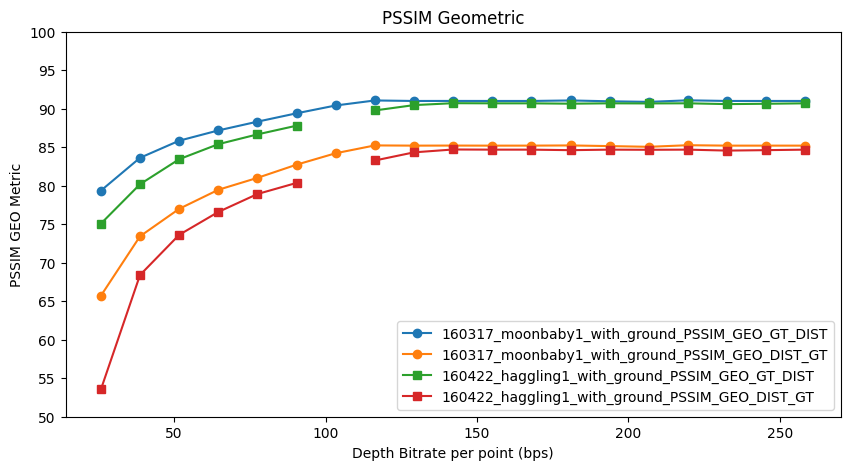
\includegraphics[width=0.8\columnwidth]{figures/depth_distortion.png}
%% %   \caption{Depth distortion vs depth bitrate.}
%% %   \label{plot:depth-distortion}
%% % \end{figure}

%% \livo exploits this to use the following bandwidth apportioning technique.
%% %
%% Suppose an RGB-D frame has $N$ points, and let $b$ be the bits per second per point for color.
%% %
%% Then, if the current total bandwidth estimate $B > 8bN$, \livo allocates $7bN$ to depth and the rest to color.
%% %
%% Otherwise, it divides $B$ in the ratio of 7:1 between color and depth.
%% %
%% For a given $B$, then, smaller point clouds (after culling) will have higher bandwidth allocated to depth and color, indicating the importance of culling.
%% %
%% %\ramesh{Add this as a possible last-minute expt?} \raj{@Ramesh should we add a discussion that bandwidth adaptation depends on the number of points. If number of points are more, it allocates more bitrate to depth by multiplying number of points with per point depth threshold and allocate rest to color. More points inside frustum -> more depth bitrate, less points -> less depth, more color.}
%% %
%% %\ramesh{Raj, please review and edit as necessary.}

%%   \squishlist
%% \item \textbf{(novel)} Bitrate splitting between color and depth. Check if we need to discuss our differences with MeshReduce.
%% \item Stream synchronization
%%   \squishend

%%   *******************************************

%%   \begin{figure}[t]
%%     \centering 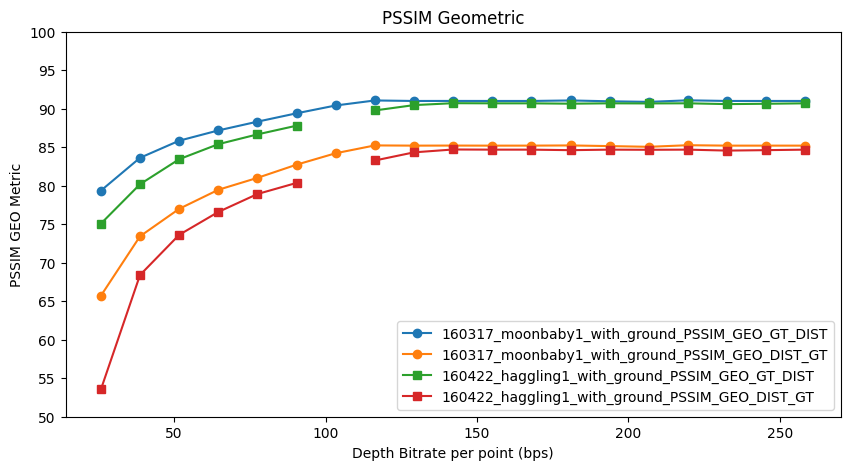
\includegraphics[width=\columnwidth]{figures/depth_distortion.png}
%%     \caption{Depth distortion vs depth bitrate.}
%%     \label{plot:depth-distortion}
%%   \end{figure}

%%   Video streaming systems maintain high QoE by adapting to bandwidth dynamics of the network. WebRTC estimates the bandwidth based on statistics collected from RTC session using Google Congestion Control (GCC) protocol~\cite{cite:gcc}. GCC feeds the estimated bitrate based on a control logic to the encoder rate control input. Using separate encoders to compress color and depth requires splitting the estimated bandwidth (also called \textit{target bitrate}) across the 2 encoders. We argue that bitrate required to compress depth is much higher than that for color, since encoding geometry requires more bits. To prove this argument, we study the effect of varying color and depth bitrate independently (fixing one and varying the other), we measure the distortion in color and depth using the PointSSIM metric~\cite{cite:point-ssim} after reconstructing the point cloud. From~\figref{plot:distortion}, we observe that variation in depth bitrate causes higher geometry error (lower PointSSIM geometry metric) than the impact of color bitrate on color metric. We also observe that PointSSIM color metric saturates around $20$ bps (bits per sec) per point, while the geometric metric saturates around depth bitrate of $140$ bps per point which is $7\times$ the color. 

%%   Based on the above empirical study, we propose a simple algorithm to split the \textit{target bitrate} $B$ between color and depth bitrates, given by $b_c$ and $b_d$, respectively. We denote $d_T$ as the threshold depth bitrate per point that saturates geometric quality metric, \ie $d_T$ is the knee of the curve~\figref{plot:depth-distortion}. Given the number of points in the predicted frustum $P$, we obtain the minimum bitrate (color + depth) $b$ that saturates the PointSSIM quality metric, which is given by the relation: \[b = d_T * P * 8 / 7\]. 

%%   If minimum bitrate $b$ is less than target bitrate $B$, we allocate $b_d = d_T * P$ as the depth bitrate and allocate rest to color, given by $b_c = B - b_d$. Otherwise, we simply allocate depth bitrate as $b_d = 6 / 7 * B$ and color bitrate as $b_c = 1 / 7 * B$.

%%   \raj{Convert into algorithm format? Do we need to compare our bitrate splitting against MeshReduce?}

%%   \raj{Do we need to elaborate on frame synchronization here?}

%% \end{comment}

%%   \parae{Determining receiver frustum.}
%%   %
%%   The frustum is determined by the pose (position and orientation) of the receiver's headset, as well as the parameters of the viewing device (such as the focal length and aspect ratio).
%%   %
%%   Today's headsets can provide continuously evolving values for these, and the receiver can transmit these to the sender.
%%   %
%%   Even so, given the feedback delay between the receiver and the sender, the latter must \textit{estimate} the frustum of the receiver at the time when the receiver views the frame.
%%   %
%%   This problem is analogous to viewport prediction in 360-degree video systems~\cite{flare, dragonfly}.
%%   %
%%   Those systems, which stream video on-demand, train predictors from user data to ensure accurate prediction in the face of the relatively long end-to-end latencies that on-demand streaming can tolerate.

%%   Prediction is qualitatively harder for volumetric video, since
%%   receivers have 6 degrees of freedom (position and rotation) instead of 3 degrees of freedom (rotation only for the viewport in 360-video).
%%   %
%%   %\harsha{I'm a bit confused: after saying above that frustum prediction is a challenge, we appear to be saying below that it is not really that hard because of low end-to-end latency.}
%%   %\rn{I guess the point is that the low latency means we can predict over very short timescales?}
%%   %
%%   However, with low end-to-end latency and, therefore, smaller prediction horizons, it may be possible to \textit{accurately} predict receiver frustums cheaply.
%%   %
%%   Indeed, \livo uses a low-overhead technique, Kalman filtering, to track and estimate the receiver frustum (\cref{ss:view-prediction}); as our results demonstrate (\cref{s:evaluation}), this can be quite effective at the timescales we target. \looseness=-1
%%   %\rn{low latency means shorter prediction horizon, right? I initially read it more so as faster feedback. More importantly, isn't the low latency also true for viewport prediction?}

%%   \parae{Culling views.}
%%   %
%%   \begin{figure}[t]
%%     \centering
%%     \begin{subfigure}[t]{0.49\columnwidth}
%%       \centering
%%       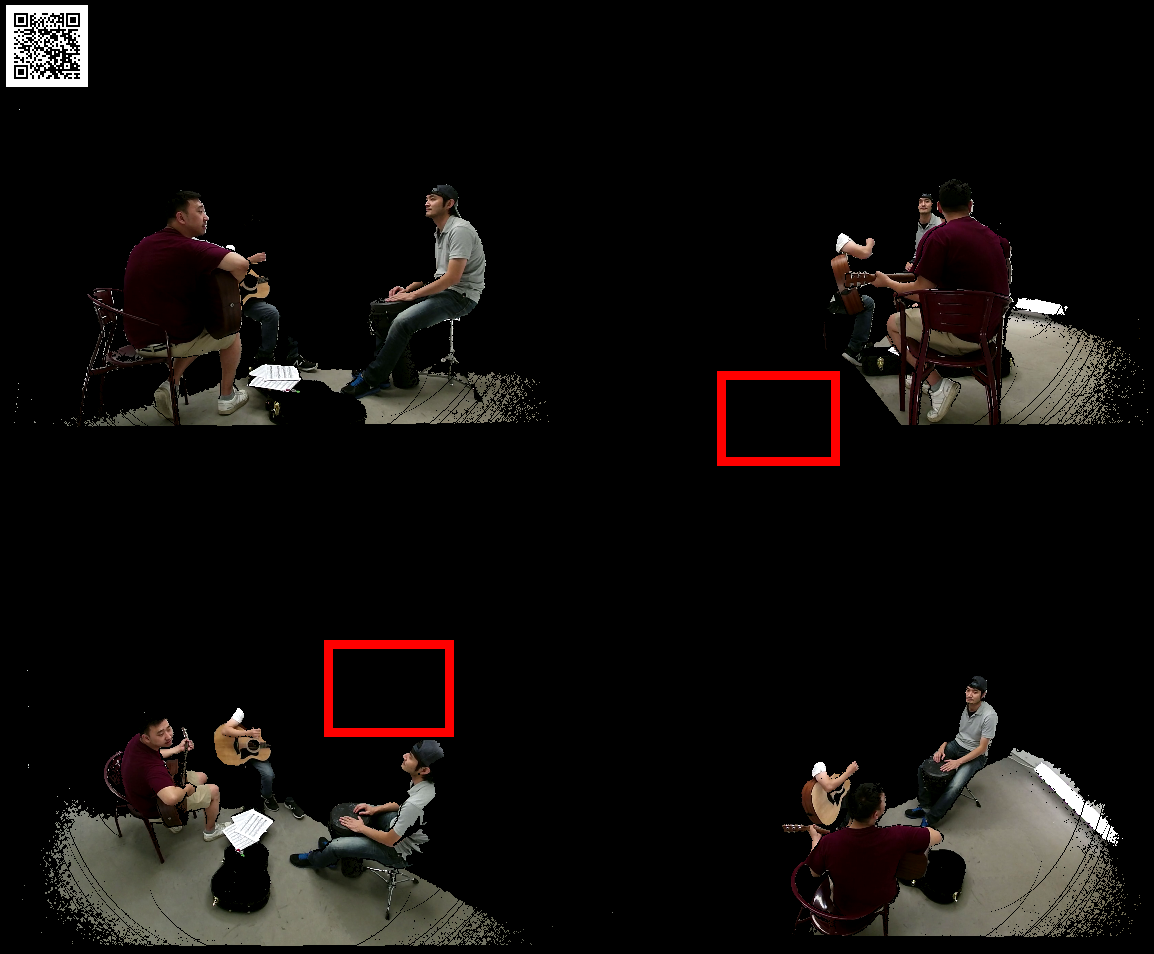
\includegraphics[width=0.9\columnwidth]{figures/10_color_bgra.png}
%%       \label{fig:tile1}
%%     \end{subfigure}
%%     \hfill
%%     \begin{subfigure}[t]{0.49\columnwidth}
%%       \centering
%%       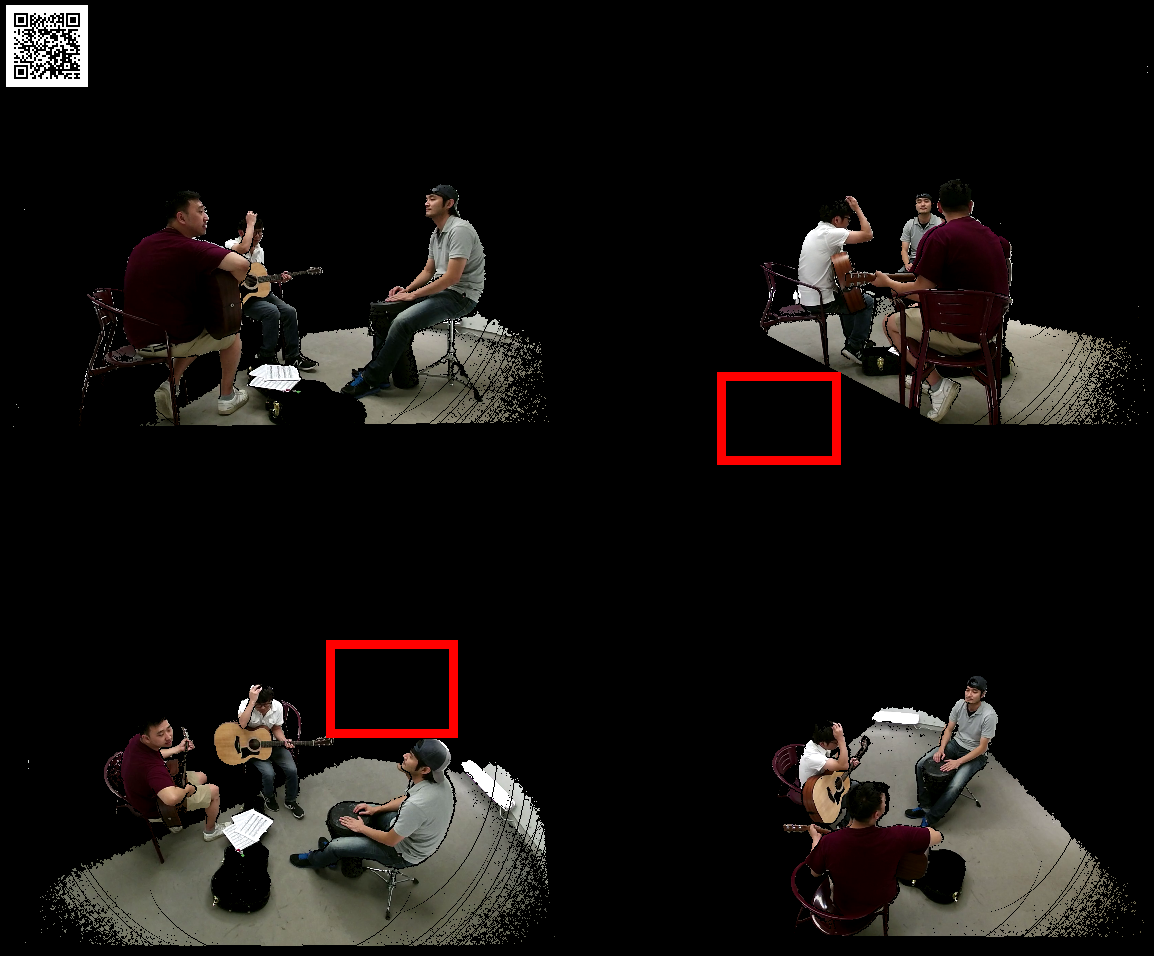
\includegraphics[width=0.9\columnwidth]{figures/20_color_bgra.png}
%%       \label{fig:tile2}
%%     \end{subfigure}
%%     \caption{The \textcolor{red}{red} boxes are culled regions with black pixels in two successive tiles that video encoders can compress efficiently.}
%%     \label{fig:cull-compress}
%%   \end{figure}
%%   %
%%   Given a frustum and a point cloud, the \textit{culled point cloud} consists of points inside the frustum.
%%   %
%%   However, RGB-D cameras do not provide point clouds explicitly; each camera produces an image, with color and depth of associated pixels.
%%   %
%%   \livo uses a fast culling technique that avoids constructing point clouds explicitly\footnote{As such, it does not need to construct spatial indices (\cref{s:challenges}), so it is more compute-efficient.}
%%   (\cref{ss:view-generation}).
%%   %
%%   All culled points in an RGB-D frame are replaced by a fixed color and depth value.
%%   %
%%   This improves compressibility, since the culled portions of the RGB-D frame have redundancy (constant color and depth), which compression algorithms can exploit (\cref{fig:cull-compress}). %\ramesh{Consider adding a simple example to illustrate this. Show two successive RGB-D frames, culled. Then highlight successive empty macroblocks and the caption can say these can be compressed efficiently.}
%%   %\raj{@Ramesh: Can you please elaborate what you mean here?}

%%   \parae{Encoding point clouds in a 2D video streams.}
%%   %
%%   Given culled frames, \livo uses standard 2D video compression techniques but must overcome two challenges.
%%   %
%%   First, video compression techniques work well to compress color in natural images.
%%   %
%%   However, RGB-D frames also contain depth information, which prior work has encoded as a separate image.
%%   %
%%   Because these approaches introduce significant distortions, \livo uses a different method, exploiting a rarely-used feature of the H.265 standard to encode depth (\cref{ss:compression}). %\ramesh{Consider including a simple experiment comparing the older real-sense depth encoding vs. the newer.}
%%   %
%%   The second challenge is to determine how to transmit the resulting \textit{two} video streams \textit{per} RGB-D camera (one for color, one for depth).
%%   %
%%   Transmitting each as a separate stream increases system complexity significantly.
%%   %
%%   Instead, \livo exploits an interesting property of RGB-D cameras like the Kinect; their resolutions are significantly less than RGB cameras for cost reasons (RGB-D cameras need depth sensors as well).
%%   %
%%   This allows \livo to encode color frames from all cameras into a single video stream, and depth frames into another\footnote{Since depth has a lower resolution than color, the color frame is downsampled to match the resolution of depth.} (\cref{ss:compression}).

%%   \parae{Apportioning available bandwidth.}
%%   %
%%   Bandwidth-adaptive video transmission for conferencing feeds bandwidth estimates to a rate-adaptive codec that attempts to compress each frame to the target bandwidth.
%%   %
%%   \livo must determine how to apportion the bandwidth estimate across the two streams: one for color frames, and the other for depth frames.
%%   %
%%   To do this, it exploits two properties: (a) beyond a certain point, allocating more bandwidth (or bits) to a pixel for depth or color does not noticeably improve \textit{objective quality}; (b) for volumetric videos, distortions in depth impact quality more than color distortions~\cite{vpcc,gpcc,pcc-future}.
%%   %
%%   \livo leverages these insights to develop an adaptive bandwidth apportionment technique (\cref{ss:bw-adaptation}). \looseness=-1



%% ********************************************

%% \raj{1 page}

%% Our approach is based on a novel combination of two insights:
%% \squishlist
%% \item Instead of synthesizing the volumetric video at the server, generate the point clouds at the client but transmit depth and color using standard video compression
%% \squishlist
%%     \item Allows us to leverage substantial investment in video compression, congestion control and live video bandwidth adaptation using quality tradeoffs.
%% \squishend

%% \item View prediction is accurate over short timescales, and server can cull views by tracking short-term history of viewer motion.
%% \squishend
	
%% \raj{At a high-level, we should explain how bandwidth adaptation works.}
	
%% Explain the architecture of the system and highlight the 3 parts of the approach: Explain overall architecture for 2-3 paragraphs with a picture.

%% ********************************************

%% We propose \livo, a live volumetric video system that leverages existing investment in live 2D video streaming and use them for 6DoF videos with carefully chosen optimizations to achieve goals - first, achieve line frame rate, preferably 30~fps; second, bandwidth adaptation with quality trade-offs; third, run within local broadband bandwidth; fourth, deployable with low software or hardware requirements. 

%% An overview of the architecture of \livo is presented in~\figref{fig:architecture_livo}. We propose an orthogonal approach compared to the strawman solution of generating and transmitting ptcl frames over the network. \livo captures RGB-D frames from multiple kinect cameras, processes the frames to reduce raw data size and compresses the frames using a pair of H.265 video encoders (2D video encoder) and transmits over the network to the receiver using WebRTC. The receiver decodes into RGB-D frames, reconstructs ptcls and renders them to the display based on the viewer's frustum. Our design decision of transmitting RGB-D frames instead of ptcl frames allow us to use 2D video encoding, which has matured for years compared to the rather nascent 3D encoders. 

%% We start to describe our design from capture to rendering (sender on the left to reciever on the right); refer to~\figref{fig:architecture_livo}. The scene is captured on the sender-side via multiple synchronized kinect cameras surrounding the scene. Each RGB-D frame captured by a camera is called a \textit{view} and all the synchronized views are assigned the same frame identifier (frame\_id). \livo can naively send all the synchronized captured RGB-D views for the same frame\_id to the receiver, but only part of the reconstructed ptcl can be viewed by the viewer which depends on the FoV. Based on this observation, the sender can send only portions the RGB-D views. The sender receives viewer's frustum for each frame rendered on the receiver. Based on the latest received frustum, the \livo predicts where the viewer might look using a \textit{Kalman Predictor}. For every pixel in both color and depth views, \livo only considers the pixels can generate a point after reconstruction that will lie inside the viewer's predicted frustum; we call this method as \textit{adaptive view culling}. This step generates new color and depth views, each corresponding to the original view (obtained from a camera) and having same resolution, which contains the original pixels that survive after culling in their original pixel locations while the culled pixels are replaced by black pixel (RGB $= (0, 0, 0$) for color and $0$ for depth. After culling, \livo stacks the culled views one after another in a grid to form one large view for color and depth separately;~\figref{fig:tiled-view}. We call each of this larger view, one for color and another for depth, as a \textit{tiled view}. For any frame, each view corresponding to a camera is always placed in the same pre-defined location in the \textit{tiled view}. This ensures 2 properties - first, all the synchronized culled views for same frame\_id are part of a single tiled view; second, the video encoder can perform motion compensation across subsequent frames, since the position of views are preserved in the \textit{tiled view}. Now, the sender uses 2 different H.265 video encoders, one each for color and depth, to compress the tiled views independently. It transmits the compressed color and depth bytestream independently through 2 WebRTC connections to the receiver.

%% The receiver decodes the bytestream separately using two H.265 decoder, one for color and another for depth respectively to their corresponding \textit{tiled view}. A \textit{tiled view} contains individual views (corresponding to each camera) synchronized, but 2 different WebRTC connections do not ensure synchronization between the color and depth tiles, \eg the receiver can receive a color tile for frame\_id $100$ and a depth tile for frame\_id $102$. The receiver needs to synchronize RGB-D tiles for downstream ptcl generation. It runs a frame synchronizer that emits a color and depth tile for the same frame\_id. The sender attaches a QR code that embeds the frame\_id to a pre-defined corner of every color and depth tiles; refer to~\figref{fig:tiled-view}. The receiver decodes the QR code to perform the tile synchronization. It decomposes a tile to it's individual views based on the pre-defined position of the views in the tile corresponding to each camera. This step is the reverse of tile generation process on the sender. Now, \livo has $N$ synchronized RGB-D views for same frame\_id. It uses the extrinsic camera calibration matrix to project each RGB-D pixel to a point in the global point cloud. The camera matrices, both instrinsic and extrinsic, are sent to the receiver. Finally, the generated ptcl is culled at the receiver based on the viewer's current frustum and rendered.

%% \end{comment}


%% First, video compression techniques work well to compress color in natural images.
%% %
%% However, RGB-D frames also contain depth information, which prior work has encoded as a separate image.
%% %
%% Because these approaches introduce significant distortions, \livo uses a different method, exploiting a rarely-used feature of the H.265 standard to encode depth (\cref{ss:compression}). %\ramesh{Consider including a simple experiment comparing the older real-sense depth encoding vs. the newer.}
%% %
%% The second challenge is to determine how to transmit the resulting \textit{two} video streams \textit{per} RGB-D camera (one for color, one for depth).
%% %
%% Transmitting each as a separate stream increases system complexity significantly.
%% %
%% Instead, \livo exploits an interesting property of RGB-D cameras like the Kinect; their resolutions are significantly less than RGB cameras for cost reasons (RGB-D cameras need depth sensors as well).
%% %
%% This allows \livo to encode color frames from all cameras into a single video stream, and depth frames into another\footnote{Since depth has a lower resolution than color, the color frame is downsampled to match the resolution of depth.} (\cref{ss:compression}).


%% \parab{Inputs and Outputs.}
%% %
%% The outputs of view culling are $N$ color and $N$ depth \textit{image frames} every inter-frame interval.
%% %
%% \livo must encode these into one or more video streams so they can be compressed using standard video compression techniques.

%%   \squishlist
%% \item Color and Depth encoding. Depth encoding using 16-bit encoder.
%% \item \textbf{(novel)} tiling leveraging 4K, RGB-D have smaller frame sizes, GPUs have parallelism for fast encoding of large frames.
%%   \squishend

%%   *******************************************

%%   \begin{figure}[t]
%%     \begin{minipage}{\columnwidth}
%%       \centering
%%       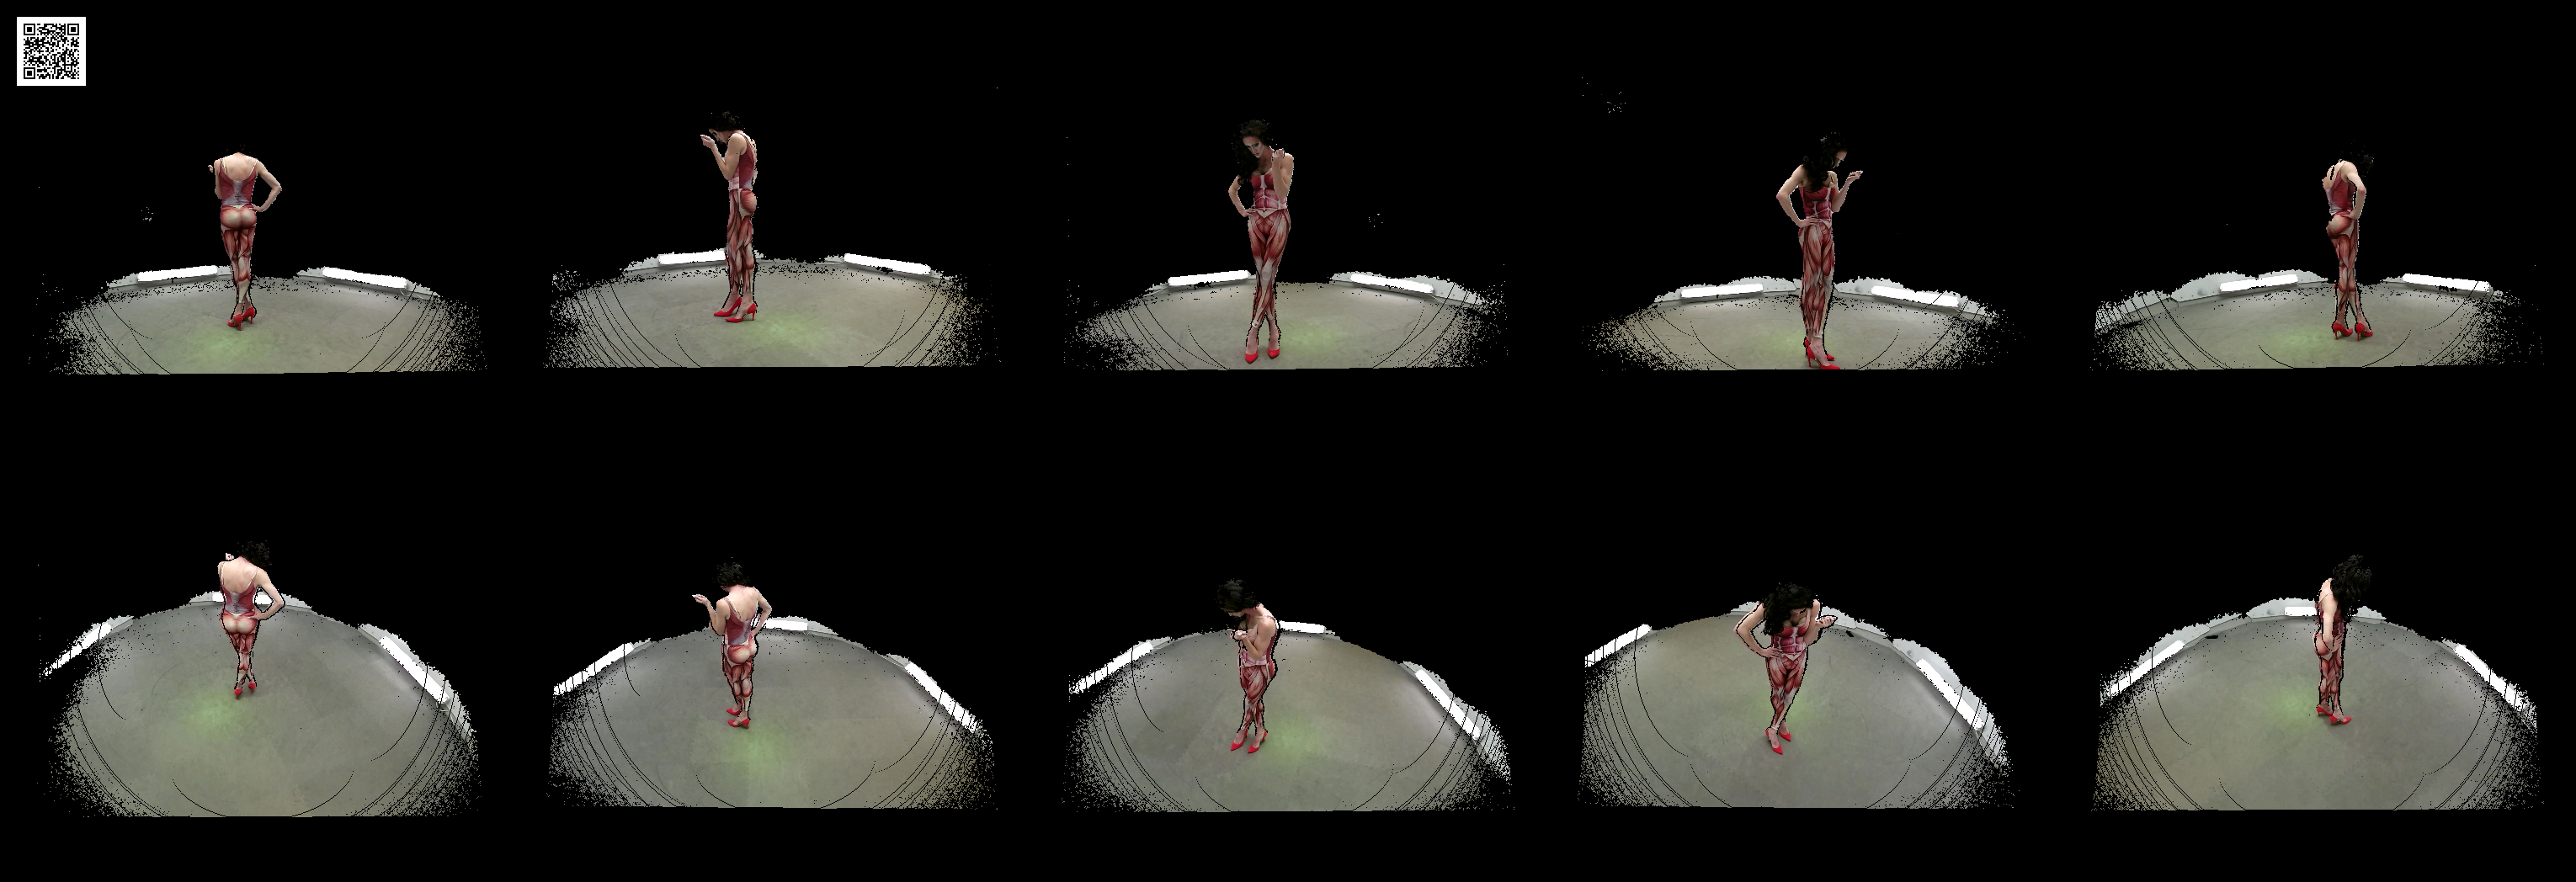
\includegraphics[width=\columnwidth]{figures/color_tiled.png}
%%     \end{minipage}
%%     \\
%%     \begin{minipage}{\columnwidth}
%%       \centering
%%       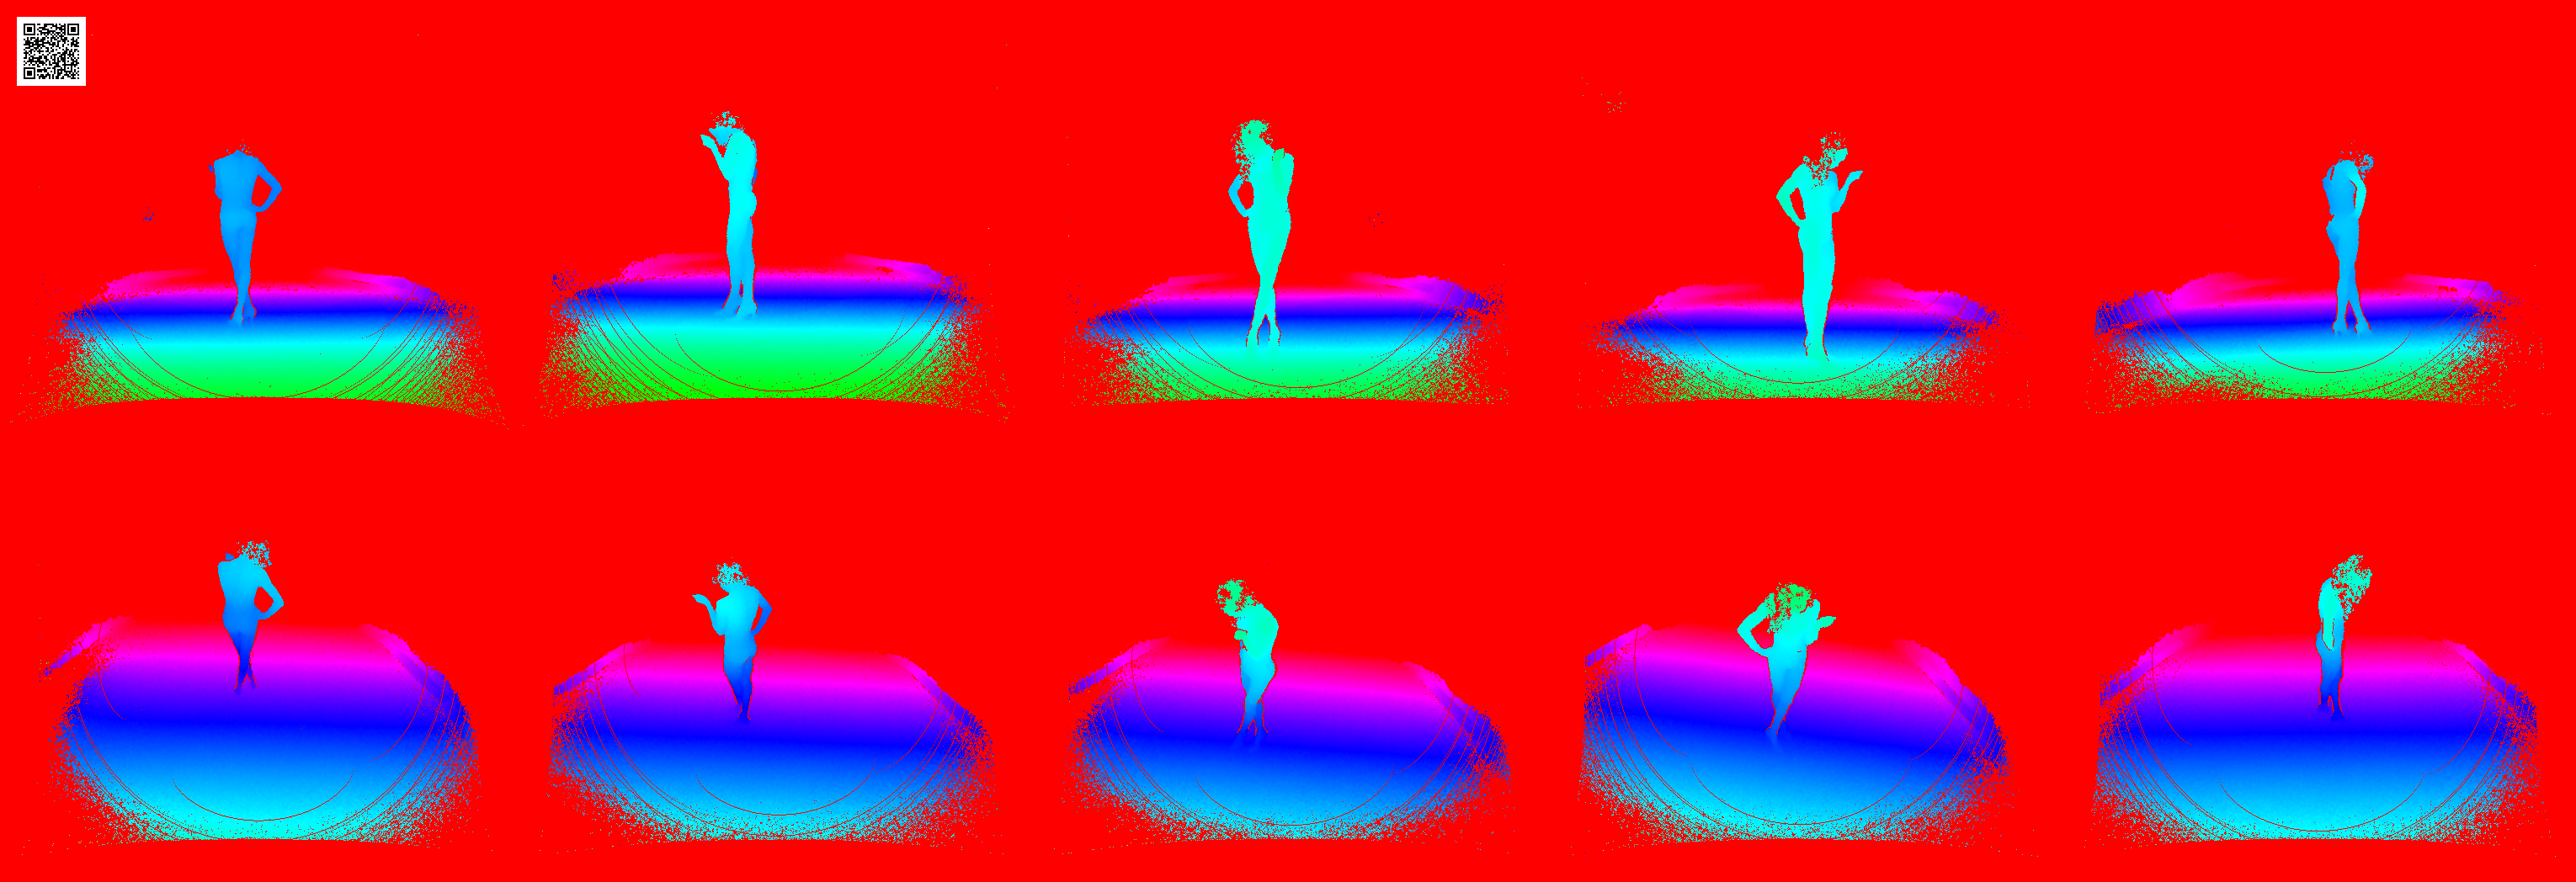
\includegraphics[width=\columnwidth]{figures/depth_tiled.png}
%%     \end{minipage}
%%     \caption{Tiled color and depth view for 10 kinect cameras.}
%%     \label{fig:tiled-view}
%%   \end{figure}

%%   The culled $N$ RGB-D views need to compressed before transmitting them to the receiver. A naive solution is to use $N$ parallel video encoders to compress color and another set of $N$ encoders to compress depth. This can leverage both intra-frame and inter-frame compression to achieve high compression ratio  at the expense of high computational overhead to run $2N$ encoders in parallel. We observe that best depth cameras available today have limited depth resolution, \eg Azure Kinect DK offers multiple depth resolutions depending on FoV and maximum range, where the most common ones are NFOV unbinned at $640 \times 576$ and WFOV $2 \times 2$ binned at $512 \times 512$. Newly released Intel RealSense D457 can support depth resolution upto $1280 \times 720$. Point cloud generation requires color and depth views to be at same resolution. Since color resolution is higher than depth, color is scaled to the depth resolution; the reverse causes depth distortion and geometric artifacts~\cite{cite:kinect-doc}. \livo ensures that RGB-D views are at same resolution after capture. In order to reduce the number of RGB-D views, we stack all the color views (likewise for depth) one after another in a grid to form a larger view; refer~\figref{fig:tiled-views}. If we use 2 tiled 4K views, one for color and another for depth, we can fit $9$ Intel RealSense cameras and $16$ Azure Kinect DK cameras, which is more than required for an affordable volumetric capture setup~\cite{cite:kinect-capture, cite:farfetchfusion, cite:holoportation}. Today, the price of these cameras are around $\$400$, so deploying more than $9$ cameras in a home or office setup seems infeasible.

%%   The $N$ cameras capture RGB-D views and transmits them to a PC over USB as an input to the sender pipeline. The sender generates 2 tiled views, one for color and another for depth. Today, video encoders have the capability to compress $4K$ video at line rate, unlike the 3D encoders, due to the availability of video encoding chipsets and graphics processors in most PC and laptops. The sender fires 2 H.265 video encoders to compress color and depth separately. The tiling scheme preserves locations of RGB-D views across frames, \ie the view of first camera is always located at the top left corner in the first rows, second is stacked after the first, till the first row is exhausted, then the next views are stacked in the row below; refer to~\figref{fig:tiled-views}. Though the sender runs only one encoder for color (another for depth), the encoder can perform motion compensation in the same way as running $N$ encoders in parallel where each encoder is responsible for a single view.

%%   \begin{figure}[t]
%%     \centering
%%     \includegraphics[width=\textwidth]{example-image-duck}
%%     \caption{\raj{Plot showing geometry error between depth to RGB quantization vs naive 16-bit encoding vs scaled 16-bit encoding}}
%%     \label{plot:depth-encoding}
%%   \end{figure}

%%   Video encoders are designed to compress color, where every pixel has 8-bits in each of the 3 channels (4 channels with transparency). Since depth is a 16-bit single channel image, it's not straightforward to use the same encoder for this purpose. Recent works like Starline~\cite{cite:starline} and FarfetchFusion~\cite{cite:farfetch-fusion} have used 10-bit color encoder by storing depth in 10-bit Y channel and keeping U and V channels as constant. This method suffices for portrait 3D videos, as the use-case in these works, it limits full 6-DoF experience since the cameras need to be within 1 meter ($2^{10} = 1024$~mm) range or giveaway millimeter range accuracy by scaling the depth to fit within 10 bit. Another approach suggested by Intel RealSense SDK is to quantize the 16-bit depth value to 3 channel RGB image~\cite{cite:realsense-doc}, but the method suffers from loss in geometry. We found that H.265 encoder can support 3 channel 16-bit encoding~\cite{cite:nvenc} in YUV format. \livo uses this variant of the encoder by storing the 16-bit depth pixel value to the Y channel and U, V channels remain constant. But, this method suffers from large geometrical errors in the form of artifacts since the encoder compresses nearby depth values to same quantization level, resulting in lossy depth. \raj{Do we need a figure to demonstrate this effect?} We observe that current depth cameras have maximum depth range of 5-6~meters~\cite{cite:kinect-spec, cite:realsense-spec}. To prevent encoder to quantize nearby depth to the same level after compression, we scale the depth pixels from $0 - 6000$ (6000 mm = 6~meters) to $0 - 2^{16}-1$ range. We show in~\figref{plot:depth-encoding} that this scheme has least geometry error than the other 2 schemes.

%% \end{comment}

%% For a given frame, the optimal split can be obtained by measuring the quality metric, PointSSIM in this case, between the ground truth and the distorted point cloud. 
%% %
%% Since PointSSIM computes the color and depth quality separately, the optimal split is the one that maximizes both PointSSIM color and depth. 
%% %
%% But, finding the optimal split is infeasible in live streaming, since the ground truth is not available on the receiver to compute PointSSIM.
%% %
%% An alternate approach is to compute it on sender-side, but this will incur computational cost of generating both the ground truth point cloud and reconstructing point cloud after decoding.
%% %
%% Moreover, PointSSIM takes more than a second and is computationally heavier compared to 2D image metrics, thus unsuitable for our use-case.

%% \parab{Naive approach.}
%% While the general problem is hard, \livo can apportion bandwidth unequally based on two intuitive observations.
%% %
%% First, humans are much more sensitive to depth than to color errors~\cite{graphsim}.
%% %
%% Thus, allocating more bandwidth to the depth stream rather than the color stream makes sense.
%% %
%% But how much more?

%% To determine this, we can conduct a study where we can fix color (resp. depth) and vary the rate allocated to depth (resp. color), the \textit{reconstruction quality} of the stream will saturate beyond a certain point.
%% %
%% This makes intuitive sense: quality will reach a point of diminishing returns with increasing bandwidth allocation.
%% %
%% We can empirically find the saturation point for both depth and color and call our split to the be ratio of the saturation points.
%% %
%% This scheme suffers from 2 problems.
%% %
%% First, the split is fixed based on a study of videos, which might be sub-optimal for any scene.
%% %
%% Second, scene complexity in the depth and color isn't captured, such as new objects entering/leaving, dynamism in the scene objects.
